% Proposal penelitian, format naskah akademik FILKOM UB (template di ../template-latex).
% Berkas ini hanya merangkai bagian-bagian; SELURUH format ada di gaya/ubtesis.sty.
% Kompilasi: latexmk main.tex   (pdfLaTeX + biber)
\documentclass[12pt,a4paper,oneside]{report}
\usepackage{gaya/ubtesis}
\usepackage{makecell}  % sel tabel bertumpuk
\addbibresource{referensi.bib}

% ------------------------------------------------------------- data sampul
\newcommand\judul{Pengaruh Mesin OCR dan Embedding Teks terhadap Pemanfaatan
  Modalitas Teks pada Klasifikasi Dokumen Multimodal}
\newcommand\jenisnaskah{PROPOSAL PENELITIAN}
\newcommand\matakuliah{ANALISIS \& PEMROSESAN DATA MULTIMODAL}
\newcommand\pengampu{Dr. Eng. Fitra Abdurrachman Bachtiar, S.T., M.Eng.}
\newcommand\programstudi{PROGRAM STUDI MAGISTER ILMU KOMPUTER}
\newcommand\departemen{DEPARTEMEN TEKNIK INFORMATIKA}
\newcommand\fakultas{FAKULTAS ILMU KOMPUTER}
\newcommand\universitas{UNIVERSITAS BRAWIJAYA}
\newcommand\kota{MALANG}
\newcommand\tahun{2026}
% Anggota kelompok, diurutkan menurut NIM.
\newcommand\anggota{%
  Yulian Anggreaif Rudamaga & 256150100011001 \\
  Zalzabila Rani             & 256150100011008 \\
  Ramadhani Al-Qadri         & 256150100011010 \\}

\begin{document}
% ------------------------------------------------------------- halaman awal
\margininduk
\pagenumbering{roman}
% Sampul. Susunannya mengikuti sampul Progress 1 kelompok (mata kuliah di atas,
% anggota kelompok dengan NIM, dosen pengampu), dengan huruf dan blok institusi
% mengikuti template FILKOM UB. Tanpa nomor halaman, terhitung halaman i.
\begin{titlepage}
\thispagestyle{empty}
\setlength{\parskip}{0pt}
\centering
\vspace*{-0.6cm}
{\bfseries\ukuran{14}\matakuliah\par}
\vspace{0.7cm}
{\bfseries\ukuran{16}\judul\par}
\vspace{0.6cm}
{\bfseries\ukuran{14}\jenisnaskah\par}
\vspace{1.3cm}
\includegraphics[width=4.5cm]{logo-ub}\par
\vspace{1.3cm}
{\ukuran{12}Disusun oleh:\par\vspace{0.25cm}
 \begin{tabular}{@{}l@{\quad:\quad}l@{}}\anggota\end{tabular}\par}
\vspace{1.1cm}
{\ukuran{12}Dosen Pengampu:\par
 \pengampu\par}
\vfill
{\bfseries\ukuran{14}\programstudi\par
 \departemen\par
 \fakultas\par
 \universitas\par
 \kota\par
 \tahun\par}
\vspace{0.16cm}
\end{titlepage}
\setcounter{page}{2}

\daftarisi
\daftartabel
\daftargambar
\daftarlampiran

% ------------------------------------------------------------- isi
\marginisi
\clearpage
\pagenumbering{arabic}
\chapter{Pendahuluan}\label{bab:pendahuluan}

\section{Latar Belakang}\label{sec:latar-belakang}

Dokumen hasil pindai menyimpan informasi pada dua lapis sekaligus. Lapis pertama adalah
\textbf{tata letak}: posisi blok, kerapatan tulisan, tabel, kop surat, dan tanda tangan.
Lapis kedua adalah \textbf{isi tekstual}: kata-kata seperti \textit{Dear Sir},
\textit{Memorandum}, atau \textit{Curriculum Vitae} yang langsung menandai jenis dokumen.
Lapis pertama terlihat langsung pada citra. Lapis kedua tersembunyi di dalam piksel dan
harus dikeluarkan lebih dulu melalui \textit{optical character recognition} (OCR).
Karena teksnya diturunkan dari citra, \textbf{mutu modalitas teks dibatasi oleh mutu
OCR-nya}.

Pada laporan Progress~1, kelompok kami mengusulkan replikasi model dua cabang
\textcite{audebert2020}. Model ini menggabungkan MobileNetV2 untuk citra halaman dengan
FastText dan CNN~1D untuk teks hasil Tesseract. Replikasi diuji pada dataset Tobacco3482,
dan Progress~1 mengajukan tiga pertanyaan:
\begin{enumerate*}[label=(\alph*)]
  \item seberapa besar akurasi naik bila kedua modalitas digabung;
  \item strategi penggabungan mana yang bekerja; dan
  \item apakah model gabungan sungguh memakai kedua sumber.
\end{enumerate*}

Sejak Progress~1, replikasi tersebut telah dijalankan penuh, dan ketiga pertanyaan itu
telah terjawab (Subbab~\ref{sec:studi-pendahuluan}). Jawaban pertanyaan (c) yang paling
menentukan arah penelitian ini. Secara angka, replikasi berhasil: model gabungan
mencapai akurasi 0,834, di atas baseline citra (0,809) dan baseline teks (0,727). Namun
ketika seluruh masukan teks dinolkan saat inferensi, akurasinya hanya turun
\textbf{0,0015}. Model gabungan itu ternyata \textbf{diam-diam unimodal}: kenaikan
akurasinya tidak berasal dari teks. Padahal komplementaritas kedua modalitas jelas ada,
karena 8,9\% dokumen uji hanya dapat diklasifikasikan dengan benar melalui teks.

Temuan ini menyingkap kelemahan cara bidang ini melaporkan hasil. Studi fusion teks--citra
umumnya hanya melaporkan akurasi gabungan. Padahal, seperti ditunjukkan replikasi kami,
akurasi gabungan yang tinggi tidak membuktikan bahwa kedua modalitas benar-benar dipakai.

Studi terkini mewarisi kelemahan yang sama dan menambah satu kelemahan lain.
\textcite{kashyap2026} menggabungkan EfficientNetB3 dan BERT, dan melaporkan akurasi
92,00\% pada Tobacco3482. Akan tetapi, mesin OCR yang menghasilkan teksnya hanya disebut
\enquote{mesin OCR komersial}, tanpa nama. Akibatnya, keunggulan cabang teks mereka tidak
dapat dipisahkan dari mesin OCR yang tidak diketahui itu.

Di tingkat bidang, meta-analisis atas 139 studi oleh \textcite{mironczuk2026} menemukan
bahwa fusion multimodal menaikkan akurasi rata-rata 5,28 poin. Namun meta-analisis itu
\emph{tidak dapat} mengontrol kualitas OCR, karena studi primer jarang melaporkannya.
Hanya 11,8\% studi multimodal yang memakai uji statistik. Perbandingan mesin OCR yang ada,
misalnya \textcite{francis2025}, mengukur ketepatan OCR itu sendiri, bukan dampaknya pada
tugas lanjutan. Padahal galat OCR terbukti merambat ke tugas berikutnya
\parencite{zhang2025}.

Tanggapan dosen pengampu atas Progress~1 mengarahkan penelitian ini ke celah tersebut.
Arahan itu meliputi eksplorasi mesin OCR selain Tesseract (EasyOCR, PaddleOCR,
Keras-OCR), eksplorasi pada sisi embedding, perumusan celah penelitian yang eksplisit,
dan referensi utama yang terbit paling awal tahun 2025. Riwayat lengkap pemilihan
referensi dan tanggapan dosen dicatat pada Lampiran~\ref{lam:riwayat}.

Penelitian ini karena itu menjadikan \textbf{mesin OCR} dan \textbf{embedding teks}
sebagai variabel. Pengaruh keduanya diukur bukan hanya terhadap akurasi, tetapi juga
terhadap \emph{seberapa jauh model gabungan benar-benar memakai} modalitas teks.

\section{Rumusan Masalah}\label{sec:rumusan-masalah}

\begin{enumerate}[label=RM\arabic*.,leftmargin=1.2cm,labelwidth=1.2cm]
  \item Seberapa besar pilihan mesin OCR (Tesseract, EasyOCR, PaddleOCR) mengubah akurasi
  cabang teks pada klasifikasi dokumen Tobacco3482?
  \item Apakah embedding kontekstual (BERT) memperkecil selisih antar-mesin OCR
  dibandingkan embedding subword statis (FastText)? Dengan kata lain, adakah interaksi
  antara mesin OCR dan jenis embedding?
  \item Apakah cabang teks yang lebih kuat membuat model gabungan lebih
  \emph{memakai} modalitas teks? Apakah aturan fusion rata-rata logit lebih tahan
  terhadap cabang yang timpang dibandingkan fusion tingkat fitur?
\end{enumerate}

\section{Tujuan Penelitian}\label{sec:tujuan}

\begin{enumerate}[label=T\arabic*.,leftmargin=1.2cm,labelwidth=1.2cm]
  \item Mengukur pengaruh mesin OCR terhadap akurasi dan macro F1 cabang teks, disertai
  uji statistik antar-mesin.
  \item Mengukur interaksi mesin OCR dan jenis embedding melalui desain faktorial.
  \item Mengukur pemanfaatan modalitas teks pada model gabungan melalui uji
  \textit{missing modality}, serta membandingkan aturan rata-rata logit
  \parencite{kashyap2026} dengan fusion tingkat fitur.
\end{enumerate}

\section{Manfaat Penelitian}\label{sec:manfaat}

\begin{enumerate}
  \item \textbf{Manfaat akademik.} Penelitian ini menyediakan protokol evaluasi fusion
  yang melampaui akurasi gabungan: uji \textit{missing modality}, beberapa seed, dan uji
  statistik. Protokol ini menjawab kekurangan pelaporan yang diidentifikasi
  \textcite{mironczuk2026}.
  \item \textbf{Manfaat praktis.} Penelitian ini memberi dasar empiris untuk memilih mesin
  OCR open-source pada sistem klasifikasi dokumen. Dasar ini diukur dari dampaknya pada
  klasifikasi, bukan dari ketepatan OCR semata.
  \item \textbf{Bahan tahap lanjutan.} Kotak posisi teks dari setiap mesin OCR disimpan
  sejak awal sebagai bahan tahap berikutnya, yaitu teks sebagai objek
  (Subbab~\ref{sec:lanjutan}).
\end{enumerate}

\section{Batasan Masalah}\label{sec:batasan}

\begin{enumerate}
  \item Dataset yang dipakai hanya Tobacco3482 (3.482 dokumen, 10 kelas). RVL-CDIP
  \parencite{harley2015} tidak dipakai karena ukurannya ($\pm$400.000 dokumen) di luar kemampuan perangkat yang
  tersedia. Akibatnya, angka penelitian ini \textbf{tidak sebanding langsung} dengan
  \textcite{kashyap2026}, yang melatih modelnya pada RVL-CDIP.
  \item Kualitas OCR diukur melalui proksi. Tobacco3482 tidak memiliki transkripsi acuan,
  sehingga \textit{character error rate} tidak dapat dihitung.
  \item Cabang citra dibuat tetap (MobileNetV2) di semua kondisi, supaya perbedaan hasil
  hanya berasal dari sisi teks.
  \item Seluruh komputasi dijalankan pada satu laptop dengan GPU 4~GB VRAM.
\end{enumerate}

\chapter{Landasan Kepustakaan}\label{bab:landasan}

\section{Kajian Pustaka}\label{sec:kajian-pustaka}

\subsection{Fusion Teks dan Citra pada Tobacco3482}

\textcite{audebert2020} merancang jaringan dua cabang yang dapat dilatih
\textit{end-to-end}:
\begin{itemize}
  \item cabang citra: MobileNetV2 dengan masukan $384\times384$;
  \item cabang teks: FastText dan CNN~1D atas teks hasil Tesseract~4;
  \item fusion: konkatenasi vektor fitur kedua cabang.
\end{itemize}
Pada Tobacco3482, fusion mencapai akurasi 87,8\%, di atas baseline citra (84,5\%) dan
baseline teks (73,8\%). Hasilnya dirata-ratakan atas tiga run tanpa simpangan baku.
Penulis juga melaporkan bahwa penjumlahan fitur berada di bawah baseline citra, tetapi
tanpa menyertakan angkanya. Di bagian penutup, penulis menyebut embedding yang tahan derau
OCR sebagai arah penelitian lanjutan. Paper inilah yang direplikasi pada studi
pendahuluan kami (Subbab~\ref{sec:studi-pendahuluan}).

\textcite{kashyap2026} adalah penerus langsung pendekatan tersebut dan menjadi
\textbf{referensi utama} penelitian ini. Ada empat perbedaan dari Audebert:
\begin{itemize}
  \item cabang citra memakai EfficientNetB3 dengan masukan $300\times300$;
  \item cabang teks memakai BERT-base;
  \item fusion dilakukan di tingkat keputusan, berupa rata-rata logit tanpa bobot;
  \item kedua cabang di-\textit{fine-tune} pada $\pm$320.000 dokumen RVL-CDIP, lalu
  Tobacco3482 dipakai hanya sebagai data uji.
\end{itemize}
Akurasi yang dilaporkan 93,06\% pada RVL-CDIP dan 92,00\% pada Tobacco3482.

Pembacaan teks lengkap paper tersebut menghasilkan tiga catatan:
\begin{enumerate}
  \item Mesin OCR-nya hanya disebut \enquote{mesin OCR komersial}, tanpa nama.
  \item Angka Tobacco3482 tidak konsisten dengan protokolnya sendiri. Kelas Note dan
  Report tidak ada di RVL-CDIP, sehingga akurasi maksimum pada 10 kelas hanya 86,6\%.
  Perhitungannya ada di Lampiran~\ref{lam:kashyap}.
  \item Hasil dilaporkan dari satu run tanpa uji statistik.
\end{enumerate}
Penulis sendiri menyebut pembobotan modalitas adaptif dan kondisi degradasi OCR yang
parah sebagai arah lanjutan. Keduanya bersinggungan langsung dengan penelitian ini.

\subsection{Gambaran Bidang: Meta-analisis Fusion untuk Klasifikasi Dokumen}

\textcite{mironczuk2026} menganalisis 139 studi primer fusion multimodal dan multiview
untuk klasifikasi dokumen. Fusion multimodal menaikkan akurasi rata-rata 5,28 poin
($p = 0{,}0016$). Namun efeknya terhadap F1 tidak signifikan secara statistik.

Tiga temuan lain dari review ini relevan langsung untuk penelitian ini:
\begin{enumerate}
  \item Hanya 11,8\% studi multimodal yang memakai uji statistik.
  \item Kualitas data, termasuk galat OCR, diakui sebagai sumber heterogenitas yang
  \emph{tidak dapat dikontrol} dalam meta-analisis, karena studi primer tidak
  melaporkannya.
  \item Penulis menganjurkan pelaporan baseline unimodal, F1 untuk data timpang, dan
  ablasi lengkap untuk setiap modalitas yang ditambahkan.
\end{enumerate}

\subsection{Perbandingan Mesin OCR dan Dampaknya pada Tugas Lanjutan}

\textcite{francis2025} membandingkan tujuh mesin OCR, termasuk Tesseract, EasyOCR,
PaddleOCR, dan Keras-OCR, pada citra campuran: dokumen cetak, layar, struk, dan ekspresi
matematika. PaddleOCR mencatat akurasi tertinggi (0,7136), diikuti EasyOCR (0,6953),
Tesseract (0,6868), dan Keras-OCR (0,6784). Selisihnya kecil, sekitar 3,5 poin. Yang
diukur di sana adalah ketepatan OCR itu sendiri, bukan dampaknya pada tugas yang
memakai teks hasil OCR.

Dampak semacam itu diukur oleh \textcite{zhang2025} untuk sistem
\textit{retrieval-augmented generation}. Mereka menyusun tolok ukur OHRBench dari 8.561
citra dokumen. Galat OCR dipilah menjadi derau semantik (kata salah baca) dan derau
format (struktur tabel atau rumus rusak). Keduanya terbukti menurunkan kinerja tugas
lanjutan. Untuk klasifikasi dokumen, pengukuran serupa belum kami temukan.

\subsection{Ketahanan Embedding terhadap Derau OCR}

\textcite{michail2025} menunjukkan bahwa model embedding standar melemah pada teks hasil
OCR, karena derau OCR jarang muncul dalam data pelatihannya. Ketahanannya dapat
dipulihkan dengan cara yang murah: \textit{fine-tuning} memakai teks yang diberi derau
karakter buatan dan \textit{loss} kontrastif, tanpa data berlabel dari domain sasaran.
Temuan ini mendasari sumbu embedding dalam penelitian ini. FastText menangani derau OCR
secara struktural melalui \textit{subword}, sedangkan BERT menanganinya melalui
tokenisasi WordPiece dan konteks kalimat.

\subsection{Jalan Pintas pada Tobacco3482}

\textcite{larson2025} menunjukkan bahwa dokumen RVL-CDIP dan Tobacco3482 bercap
\textbf{kode ID} arsip. Model sederhana yang hanya memakai fitur dari kode ID itu sudah
mencapai $\pm$60\% akurasi di Tobacco3482. Pada RVL-CDIP, classifier mutakhir kehilangan
11 poin akurasi setelah kode ID dihapus.

Kode ID ini terlihat pada contoh dokumen di Gambar~\ref{fig:contoh-pasangan}, misalnya
\texttt{00625137} dan \texttt{CTR CONTRACTS 023247}. Temuan ini menjadi kontrol wajib
pada tahap lanjutan yang memperlakukan teks sebagai objek berposisi
(Subbab~\ref{sec:lanjutan}).

\subsection{Posisi Penelitian}

Tabel~\ref{tab:posisi} memetakan studi-studi di atas terhadap lima aspek yang menjadi
fokus penelitian ini.

\begin{table}[H]
  \centering
  \caption{Posisi penelitian terhadap studi terkait}
  \label{tab:posisi}
  \fontsize{10}{12}\selectfont
  \begin{tabularx}{\textwidth}{|>{\raggedright\arraybackslash}X|c|c|c|c|c|}
    \hline
    \textbf{Studi} & \textbf{\makecell{Mesin OCR\\disebut}} &
    \textbf{\makecell{$>1$\\mesin OCR}} & \textbf{\makecell{Variasi\\embedding}} &
    \textbf{\makecell{Uji missing\\modality}} & \textbf{\makecell{Uji\\statistik}} \\ \hline
    \textcite{audebert2020} & \checkmark & -- & MLP vs CNN & -- & -- \\ \hline
    \textcite{kashyap2026} & -- & -- & -- & -- & -- \\ \hline
    \textcite{francis2025} & \checkmark & \checkmark\ (7) &
    \multicolumn{3}{c|}{tanpa tugas klasifikasi} \\ \hline
    \textbf{Penelitian ini} & \checkmark & \checkmark\ (3) & FastText, BERT &
    \checkmark & \checkmark \\ \hline
  \end{tabularx}
  \sumber{Dirangkum dari studi yang dirujuk.}
\end{table}

\section{Dasar Teori}\label{sec:dasar-teori}

\subsection{Optical Character Recognition}

OCR modern umumnya bekerja dalam dua tahap: \textbf{deteksi} wilayah teks pada citra,
lalu \textbf{pengenalan} karakter di dalam setiap wilayah. Ketiga mesin yang diuji
berbeda pada kedua tahap tersebut.

\textbf{Tesseract} \parencite{smith2007} memulai dengan analisis tata letak halaman untuk
menemukan blok, baris, dan kata, lalu mengenali teksnya. Sejak versi 4, pengenalannya
memakai jaringan LSTM yang membaca setiap baris sebagai sekuens. Konfigurasi
\texttt{-{}-psm 3} berarti segmentasi halaman otomatis penuh tanpa deteksi orientasi.
Konfigurasi inilah yang dipakai QS-OCR \parencite{qsocr}. Keluarannya mengikuti urutan baca
Tesseract sendiri, yaitu blok, paragraf, baris, lalu kata.

\textbf{EasyOCR} \parencite{easyocr} mendeteksi teks dengan CRAFT \parencite{baek2019}. CRAFT
memprediksi wilayah setiap karakter dan keterkaitan antar-karakter, lalu menggabungkannya
menjadi kotak kata atau baris. Pengenalannya memakai CRNN \parencite{shi2017}, yang terdiri
atas tiga bagian:
\begin{itemize}
  \item ekstraktor fitur konvolusi;
  \item LSTM dua arah untuk pelabelan sekuens;
  \item dekoder \textit{connectionist temporal classification} (CTC).
\end{itemize}

\textbf{PaddleOCR} \parencite{paddleocr} menyusun pipeline dari modul-modul terpisah:
klasifikasi orientasi dokumen, koreksi distorsi, deteksi baris teks, klasifikasi
orientasi baris, dan pengenalan teks. Modul orientasi dan koreksi distorsi bersifat
opsional. Penelitian ini memakai pasangan model deteksi dan pengenalan PP-OCRv5
\textit{mobile}.

Mesin berbasis kotak seperti EasyOCR dan PaddleOCR tidak menjamin urutan baca. Urutan
itu harus direkonstruksi dari posisi kotak (Subbab~\ref{sec:metode-ocr}).

\subsection{Representasi Kata}

\textbf{FastText} \parencite{bojanowski2017} merepresentasikan kata $w$ sebagai jumlah
vektor seluruh \textit{n-gram} karakternya:
\begin{equation}\label{eq:fasttext}
  \mathbf{u}_w = \sum_{g \in \mathcal{G}_w} \mathbf{z}_g
\end{equation}
dengan $\mathcal{G}_w$ himpunan \textit{n-gram} karakter kata $w$ beserta kata itu
sendiri, dan $\mathbf{z}_g$ vektor untuk \textit{n-gram} $g$. Karena itu, kata yang rusak
akibat OCR, misalnya \texttt{Tospacco}, tetap mendapat vektor yang dekat dengan kata
aslinya, karena keduanya berbagi banyak \textit{n-gram}.

\textbf{BERT} \parencite{devlin2019} adalah encoder Transformer dua arah yang dilatih awal
dengan tugas \textit{masked language modelling}. Teks dipecah menjadi sub-kata dengan
tokenisasi WordPiece, dan vektor setiap token bergantung pada konteks kalimatnya.
Panjang masukan dibatasi 512 token. Untuk klasifikasi, representasi token khusus
\texttt{[CLS]} dilewatkan ke lapisan klasifikasi, dan seluruh model di-\textit{fine-tune}.

\subsection{Arsitektur Konvolusi}

\textbf{CNN~1D untuk teks} \parencite{kim2014} menggeser filter konvolusi di sepanjang
sekuens vektor kata, lalu meringkasnya dengan \textit{max-pooling} terhadap waktu. Filter
dengan lebar $k$ berfungsi sebagai pendeteksi frasa sepanjang $k$ kata. Model ini peka
terhadap \textbf{urutan} kata, berbeda dari rata-rata vektor kata.

\textbf{MobileNetV2} \parencite{sandler2018} adalah CNN citra berbiaya rendah. Blok
penyusunnya adalah \textit{inverted residual} dengan \textit{linear bottleneck}: kanal
diekspansi dengan konvolusi $1\times1$, difilter dengan konvolusi \textit{depthwise}
$3\times3$, lalu diproyeksikan kembali tanpa aktivasi non-linear.

\subsection{Strategi Fusion}

Fusion dapat dilakukan pada tingkat fitur atau tingkat keputusan
\parencite{baltrusaitis2019}. Misalkan $\mathbf{v}_t, \mathbf{v}_v \in \mathbb{R}^{d}$
adalah vektor fitur cabang teks dan citra, dan $\mathbf{z}_t, \mathbf{z}_v \in
\mathbb{R}^{C}$ adalah logit keduanya untuk $C$ kelas.

\textbf{Fusion tingkat fitur} menggabungkan vektor fitur lalu mengklasifikasikannya
bersama. Pada konkatenasi \parencite{audebert2020}:
\begin{equation}\label{eq:concat}
  \hat{y} = \arg\max_c \; \mathrm{MLP}\!\left([\,\mathbf{v}_t \,;\, \mathbf{v}_v\,]\right)_c
\end{equation}

\textbf{Fusion tingkat keputusan} menggabungkan keluaran setiap cabang. Pada rata-rata
logit tanpa bobot \parencite{kashyap2026}:
\begin{equation}\label{eq:logit}
  \hat{y} = \arg\max_c \; \tfrac{1}{2}\left(z_{t,c} + z_{v,c}\right)
\end{equation}
Fusion tingkat keputusan menjamin kedua cabang ikut menentukan hasil. Akibatnya, cabang
yang lemah tetap memengaruhi keputusan.

Pada fusion tingkat fitur, cabang dengan skala fitur jauh lebih besar dapat mendominasi.
Masalah ini dapat diatasi dengan \textbf{Layer Normalization} \parencite{ba2016}, yang
menormalkan setiap vektor fitur terhadap rata-rata $\mu$ dan simpangan baku $\sigma$
komponennya sendiri:
\begin{equation}\label{eq:layernorm}
  \mathrm{LN}(\mathbf{v}) = \boldsymbol{\gamma} \odot \frac{\mathbf{v} - \mu}{\sigma +
  \epsilon} + \boldsymbol{\beta}
\end{equation}
dengan $\boldsymbol{\gamma}$ dan $\boldsymbol{\beta}$ parameter yang dipelajari. LN
bekerja per sampel, sehingga tidak bergantung pada ukuran \textit{batch}.

\subsection{Metrik Evaluasi}

\textbf{Overall accuracy} (OA) adalah proporsi dokumen uji yang diklasifikasikan dengan
benar. Kelas Tobacco3482 timpang, dengan rasio kelas terbesar berbanding terkecil
5,2:1, sehingga OA cenderung didominasi kelas besar. Karena itu \textbf{macro F1} juga
dilaporkan:
\begin{equation}\label{eq:macrof1}
  \mathrm{F1}_c = \frac{2\, P_c R_c}{P_c + R_c}, \qquad
  \text{macro F1} = \frac{1}{C} \sum_{c=1}^{C} \mathrm{F1}_c
\end{equation}
dengan $P_c$ dan $R_c$ presisi dan \textit{recall} kelas $c$.

\textbf{Oracle} adalah batas atas teoretis fusion: sebuah dokumen dihitung benar bila
cabang teks \emph{atau} cabang citra mengklasifikasikannya dengan benar
\parencite{audebert2020}. Selisih antara oracle dan baseline terbaik adalah potensi yang
dapat dipanen fusion.

\textbf{Uji \textit{missing modality}} mengukur ketergantungan model gabungan pada setiap
modalitas. Caranya, masukan satu modalitas dinolkan saat inferensi:
\begin{equation}\label{eq:delta}
  \Delta_\text{teks} = \mathrm{OA}_\text{utuh} - \mathrm{OA}_\text{teks dinolkan}
\end{equation}
$\Delta_\text{citra}$ didefinisikan secara analog. $\Delta_\text{teks}$ yang mendekati nol
berarti model tidak memakai teks, berapa pun akurasinya.

\textbf{Uji McNemar} \parencite{mcnemar1947} membandingkan dua classifier pada data uji
yang sama. Uji ini dianjurkan untuk perbandingan algoritme pembelajaran oleh
\textcite{dietterich1998}. Bila $b$ adalah jumlah dokumen yang hanya benar pada classifier
pertama dan $c$ jumlah dokumen yang hanya benar pada classifier kedua:
\begin{equation}\label{eq:mcnemar}
  \chi^2 = \frac{(|b - c| - 1)^2}{b + c}
\end{equation}
Statistik ini berdistribusi $\chi^2$ dengan satu derajat bebas. Bila $b + c$ kecil,
dipakai uji binomial eksak. Untuk $m$ perbandingan sekaligus, ambang signifikansi
dikoreksi menjadi $\alpha/m$ (koreksi Bonferroni, \cite{dunn1961}).

\section{Metode yang Direncanakan}\label{sec:metode}

\subsection{Kerangka Penelitian}\label{sec:kerangka}

Kerangka penelitian ditunjukkan Gambar~\ref{fig:kerangka}.

\begin{figure}[H]
  \centering
  \resizebox{\textwidth}{!}{% Kerangka penelitian. Kotak biru = variabel yang diuji.
\begin{tikzpicture}[
  box/.style={draw, rounded corners=2pt, align=center, font=\footnotesize,
              minimum height=1.15cm, minimum width=2.35cm, inner sep=2pt, fill=white},
  var/.style={box, fill=blue!8},
  arr/.style={-{Stealth[length=2mm]}, thick}]
\node[box] (img) at (0,0) {Citra JPG\\Tobacco3482};
\node[var] (ocr) at (3.0,1.35) {\textbf{Mesin OCR}\\Tesseract,\\EasyOCR, PaddleOCR};
\node[var] (emb) at (6.5,1.35) {\textbf{Embedding}\\FastText + CNN1D,\\BERT};
\node[box] (cnn) at (4.75,-1.35) {Cabang citra\\MobileNetV2\\(tetap)};
\node[var] (fus) at (9.6,0) {\textbf{Fusion}\\rata-rata logit,\\fitur + LN};
\node[box] (eva) at (12.6,0) {OA, macro F1,\\McNemar,\\$\Delta_\text{teks}$, oracle};
\node[font=\scriptsize, text=gray, align=center] (kotak) at (3.0,2.75)
     {kotak posisi teks $\rightarrow$ tahap lanjutan};
\draw[arr] (img.north) |- (ocr.west);
\draw[arr] (img.south) |- (cnn.west);
\draw[arr] (ocr) -- (emb);
\draw[arr] (emb.east) -| (fus.north);
\draw[arr] (cnn.east) -| (fus.south);
\draw[arr] (fus) -- (eva);
\draw[-{Stealth[length=1.6mm]}, gray, dashed] (ocr.north) -- (kotak.south);
\end{tikzpicture}
}
  \caption{Kerangka penelitian; kotak biru adalah variabel yang diuji}
  \label{fig:kerangka}
\end{figure}

Penelitian terdiri atas empat langkah:
\begin{enumerate}
  \item OCR ulang seluruh citra dengan tiga mesin.
  \item Melatih cabang teks untuk setiap kombinasi mesin OCR dan embedding.
  \item Menggabungkan setiap cabang teks dengan cabang citra yang sama.
  \item Mengevaluasi akurasi sekaligus pemanfaatan modalitas.
\end{enumerate}
Cabang citra sengaja dibuat tetap, supaya setiap perbedaan hasil hanya dapat berasal dari
sisi teks.

\subsection{Dataset dan Protokol}\label{sec:dataset}

\textbf{Tobacco3482} \parencite{kumar2014} berisi 3.482 citra dokumen dalam 10 kelas:
Advertisement, Email, Form, Letter, Memo, News, Note, Report, Resume, dan Scientific.
Kelas terbesar adalah Memo (620 dokumen) dan terkecil Resume (120 dokumen). Citra diambil
dari Kaggle dalam format JPG \parencite{kaggletobacco}, yang tidak memiliki lisensi baku.

\textbf{QS-OCR-Small} \parencite{qsocr} berlisensi Apache-2.0. Isinya teks Tesseract~4
dari citra TIF asli, dan dipakai sebagai \textbf{kondisi acuan}, yaitu teks yang sama
dengan yang dipakai \textcite{audebert2020}.

Protokol pembagian data mengikuti \textcite{audebert2020}:
\begin{itemize}
  \item 800 dokumen latih per pembagian, 10\% di antaranya dipakai untuk validasi;
  \item sisanya, 2.682 dokumen, menjadi data uji;
  \item tiga pembagian acak terstratifikasi, dengan seed 42, 43, dan 44;
  \item \textbf{indeks pembagian yang sama} dipakai di semua kondisi, supaya perbedaan
  antar-kondisi tidak tercampur perbedaan data.
\end{itemize}
Pemakaian dataset dibatasi untuk keperluan akademik non-komersial, dan tidak ada berkas
dataset yang didistribusikan ulang.

\subsection{Ekstraksi OCR Multi-mesin}\label{sec:metode-ocr}

Konfigurasi setiap mesin disajikan pada Tabel~\ref{tab:mesin}.

\begin{table}[H]
  \centering
  \caption{Mesin OCR dan konfigurasinya}
  \label{tab:mesin}
  \fontsize{10}{12}\selectfont
  \begin{tabularx}{\textwidth}{|l|>{\raggedright\arraybackslash}X|l|}
    \hline
    \textbf{Mesin} & \textbf{Konfigurasi} & \textbf{Kotak teks} \\ \hline
    QS-OCR (acuan) & Tesseract 4.0-beta pada TIF asli, \texttt{-{}-oem 1 -{}-psm 3} &
    tidak tersedia \\ \hline
    Tesseract & versi 5 pada JPG, konfigurasi sama dengan QS-OCR & per kata \\ \hline
    EasyOCR & model bahasa Inggris, GPU & per baris \\ \hline
    PaddleOCR & model PP-OCRv5 \textit{mobile}, CPU, tanpa koreksi orientasi &
    per baris \\ \hline
  \end{tabularx}
\end{table}

Empat keputusan desain menyertai konfigurasi tersebut:
\begin{enumerate}
  \item \textbf{Semua mesin membaca citra JPG yang sama}, termasuk Tesseract yang
  dijalankan ulang. Selisih antara QS-OCR dan Tesseract-JPG karena itu mengukur efek
  gabungan format citra dan versi Tesseract.
  \item \textbf{Urutan baca mesin berbasis kotak direkonstruksi}: baris dari atas ke
  bawah, kata dari kiri ke kanan. Karena CNN~1D peka urutan, perbedaan urutan baca dicatat
  sebagai bagian dari efek mesin.
  \item \textbf{Teks dan kotak posisi setiap halaman disimpan}, sehingga tahap lanjutan
  tidak memerlukan OCR ulang.
  \item \textbf{Versi pustaka dan nama model dikunci serta dicatat}, karena model bawaan
  mesin OCR dapat berganti antar-versi.
\end{enumerate}

Keras-OCR disarankan dosen, tetapi dimasukkan secara bersyarat. Alasannya dijelaskan pada
risiko R3 (Subbagian~\ref{sec:risiko}).

\subsection{Proksi Kualitas OCR}\label{sec:proksi}

Tobacco3482 tidak memiliki transkripsi acuan, sehingga \textit{character error rate}
tidak dapat dihitung. Tiga proksi berikut menggambarkan keluaran OCR tanpa menilai
benar-salahnya.

\begin{enumerate}
  \item \textbf{Kata per halaman dan persentase halaman kosong.} Proksi ini menangkap
  mesin yang melewatkan blok teks.
  \item \textbf{Laju OOV.} Untuk dokumen $d$, laju OOV adalah bagian kata alfabetik dengan
  panjang minimal empat huruf yang tidak terdapat dalam daftar kata bahasa Inggris $V$
  \parencite{wordfreq}:
  \begin{equation}\label{eq:oov}
    \mathrm{OOV}(d) = \frac{\left|\{w \in d : |w| \geq 4,\; w \notin V\}\right|}
                           {\left|\{w \in d : |w| \geq 4\}\right|}
  \end{equation}
  Salah baca yang kebetulan berupa kata yang ada, misalnya \texttt{tbe} untuk
  \texttt{the}, tidak terhitung. Karena itu nilai ini adalah \emph{batas bawah} galat.
  \item \textbf{Kesepakatan antar-mesin.} Kesepakatan dua mesin diukur dengan indeks
  Jaccard atas himpunan kata ($A$ dan $B$) yang keduanya baca:
  \begin{equation}\label{eq:jaccard}
    J(A, B) = \frac{|A \cap B|}{|A \cup B|}
  \end{equation}
  Urutan kata sengaja diabaikan, karena mesin berbeda urutan baca walaupun kata yang
  dibaca sama.
\end{enumerate}

\subsection{Representasi Teks dan Citra}\label{sec:representasi}

Dua representasi teks diuji.

\textbf{FastText dan CNN~1D}, mengikuti \textcite{audebert2020}. Setiap kata dipetakan ke
vektor FastText 300 dimensi (Persamaan~\ref{eq:fasttext}). Sekuens dibatasi 500 kata,
lalu diproses CNN~1D.

\textbf{BERT-base}, mengikuti \textcite{kashyap2026}. Model ini di-\textit{fine-tune}
dengan masukan maksimum 512 token. Pelatihan memakai \textit{mixed precision} dan
akumulasi gradien supaya muat di GPU 4~GB. Bila tetap tidak muat, model diganti
DistilBERT, dan penggantian itu dicatat sebagai deviasi.

Teks masuk ke kedua representasi \textbf{tanpa} praproses gaya Kashyap, yaitu tanpa
membuang angka dan \textit{stopword}. Tujuannya agar efek embedding tidak tercampur efek
praproses.

Cabang citra memakai MobileNetV2 berbobot awal ImageNet, dengan masukan $384\times384$
dan rasio aspek di-\textit{warp}, mengikuti \textcite{audebert2020}. Cabang ini sama di
semua kondisi.

\subsection{Strategi Fusion yang Diuji}\label{sec:fusion}

Dua strategi fusion diuji.

\textbf{Rata-rata logit} (Persamaan~\ref{eq:logit}), yaitu aturan
\textcite{kashyap2026}. Strategi ini tidak memerlukan pelatihan ulang, sehingga dapat
diterapkan pada \emph{semua} kondisi.

\textbf{Fusion tingkat fitur dengan normalisasi per cabang}:
\begin{equation}\label{eq:fusionfix}
  \hat{y} = \arg\max_c \; \mathrm{MLP}\!\left([\,\mathrm{LN}(\mathbf{v}_t) \,;\,
  \mathrm{LN}(\mathbf{v}_v)\,]\right)_c
\end{equation}
Layer Normalization (Persamaan~\ref{eq:layernorm}) menyamakan skala kedua vektor fitur
sebelum digabung, supaya head klasifikasi tidak otomatis didominasi cabang yang skala
fiturnya lebih besar. Cabang teks diinisialisasi dari model teks yang sudah dilatih
sendiri, supaya kedua cabang mulai dari titik yang sama-sama terlatih.

Fusion tingkat fitur memerlukan pelatihan \textit{end-to-end} yang relatif mahal, sehingga
hanya diterapkan pada kondisi OCR terbaik dan terburuk.

\subsection{Desain Eksperimen dan Hipotesis}\label{sec:desain}

Matriks eksperimen disajikan pada Tabel~\ref{tab:desain}.

\begin{table}[H]
  \centering
  \caption{Matriks eksperimen}
  \label{tab:desain}
  \fontsize{10}{12}\selectfont
  \begin{tabularx}{\textwidth}{|l|>{\raggedright\arraybackslash}X|c|}
    \hline
    \textbf{Kelompok} & \textbf{Kondisi} & \textbf{Jumlah run} \\ \hline
    Cabang teks & 4 kondisi OCR $\times$ 2 embedding $\times$ 3 seed & 24 \\ \hline
    Cabang citra & MobileNetV2 $\times$ 3 seed & 3 \\ \hline
    Rata-rata logit & setiap model teks + cabang citra dengan seed yang sama &
    24 (tanpa pelatihan) \\ \hline
    Fusion fitur & kondisi OCR terbaik dan terburuk, FastText, seed 42 &
    2 (+4 bila waktu cukup) \\ \hline
    Uji \textit{missing modality} & setiap model fusion & tanpa pelatihan \\ \hline
  \end{tabularx}
\end{table}

\textbf{Pemeriksaan kewarasan.} Kondisi QS-OCR $\times$ FastText harus menghasilkan
akurasi cabang teks yang dekat dengan angka \textcite{audebert2020} (0,738). Bila jauh
berbeda, ada yang salah dalam pipeline, dan eksperimen dihentikan sampai penyebabnya
ditemukan.

Hipotesis dirumuskan \emph{sebelum} eksekusi, dan akan dilaporkan apa adanya, termasuk
bila keliru.

\begin{enumerate}[label=H\arabic*.,leftmargin=1.2cm,labelwidth=1.2cm]
  \item \textbf{(RM1)} Perbedaan akurasi cabang teks antar-mesin OCR bersifat nyata,
  yaitu melampaui variasi antar-seed. Mesin modern belum tentu unggul. Tobacco3482 berisi
  pindaian cetak hitam putih, yaitu kondisi tempat Tesseract paling kuat. Selain itu,
  CNN~1D peka urutan baca, yang berbeda antar-mesin.
  \item \textbf{(RM2)} BERT memperkecil selisih antar-mesin dibandingkan FastText.
  Argumen tandingannya: model bahasa standar juga melemah pada teks OCR
  \parencite{michail2025}, dan batas 512 token memotong dokumen panjang.
  \item \textbf{(RM3)} Pada fusion fitur, $\Delta_\text{teks}$ membesar seiring akurasi
  cabang teks. Rata-rata logit menjamin $\Delta_\text{teks} > 0$ secara konstruksi,
  tetapi akurasinya dapat turun bila cabang teks lemah.
\end{enumerate}

\subsection{Evaluasi dan Uji Statistik}\label{sec:evaluasi}

Setiap model dievaluasi dengan empat ukuran: OA, macro F1
(Persamaan~\ref{eq:macrof1}), F1 per kelas, dan oracle. Untuk setiap model fusion
ditambahkan $\Delta_\text{teks}$ dan $\Delta_\text{citra}$ (Persamaan~\ref{eq:delta}).

Perbandingan dua kondisi memakai uji McNemar (Persamaan~\ref{eq:mcnemar}) pada data uji
yang sama, per seed. Uji binomial eksak dipakai bila $b + c < 25$. Ada enam pasangan
kondisi OCR per jenis embedding, sehingga ambang signifikansinya dikoreksi menjadi
$0{,}05/6$. Sebuah perbedaan dinyatakan konsisten bila signifikan dan arahnya sama di
ketiga seed. Semua angka dilaporkan sebagai rata-rata $\pm$ simpangan baku tiga seed.

\section{Hasil dan Pembahasan}\label{sec:hasil}

Seluruh angka pada bagian ini berasal dari satu eksekusi penuh
\texttt{notebooks/pipeline.ipynb} dan disalin dari berkas \texttt{reports/fase2/*.csv}
yang dihasilkannya. Angka turunan (selisih, panen, korelasi) dihitung dari berkas yang
sama.

\subsection{Validitas Pipeline}\label{sec:validitas}

Pemeriksaan kewarasan lolos. Cabang teks QS-OCR mereproduksi CNN~1D Fase~1
\textbf{bit-identik} per seed (OA 0,7345 / 0,7248 / 0,7204, dengan epoch terbaik yang
sama), walaupun dilatih ulang dari nol dengan kode baru. Cabang citra mencapai
$0{,}8169 \pm 0{,}0257$, di dalam toleransi terhadap Fase~1 ($0{,}8086 \pm 0{,}0210$).
Seed 44 jelas lebih lemah (0,7808, epoch terbaik 11), sedangkan seed 42 dan 43 mencapai
0,8315 dan 0,8386.

\subsection{Analisis Data Eksploratif per Modalitas}\label{sec:eda}

Analisis ini dijalankan sebelum pelatihan apa pun, pada seluruh 3.482 dokumen. Analisis
yang memakai label (kata khas, \textit{probe}, jalan pintas kode ID) hanya dipasang pada
bagian latih seed 42, sedangkan data uji hanya dipakai untuk mengukur akurasi
\textit{probe}. Untuk teks, yang dianalisis di sini adalah kondisi acuan QS-OCR;
perbandingan antar-mesin ada pada Subbagian~\ref{sec:hasil-ocr}.

\subsubsection{Distribusi Kelas dan Pembagian Data}

Kelas Tobacco3482 timpang: Memo 620 dokumen, Email 599, Letter 567, Form 431, Report
265, Scientific 261, Advertisement 230, Note 201, News 188, dan Resume 120, sehingga rasio
kelas terbesar terhadap terkecil 5,17. Pembagian terstratifikasi menghasilkan 720 dokumen
latih, 80 validasi, dan 2.682 uji dengan komposisi kelas yang sama di ketiga seed. Resume
hanya punya 25 dokumen latih dan 3 dokumen validasi per seed, dan Note 41 dan 5.

\subsubsection{Modalitas Citra}

Citra JPG beresolusi tinggi. Lebar halaman berkisar 817 sampai 3.520 piksel dengan median
1.728 piksel. Bila halaman diasumsikan berukuran \textit{letter}, perkiraan resolusinya
96 sampai 414 dpi, median 203 dpi, dan kuartil atas 299 dpi. Statistik citra per kelas
ditunjukkan Gambar~\ref{fig:eda-citra}.

\begin{figure}[H]
  \centering
  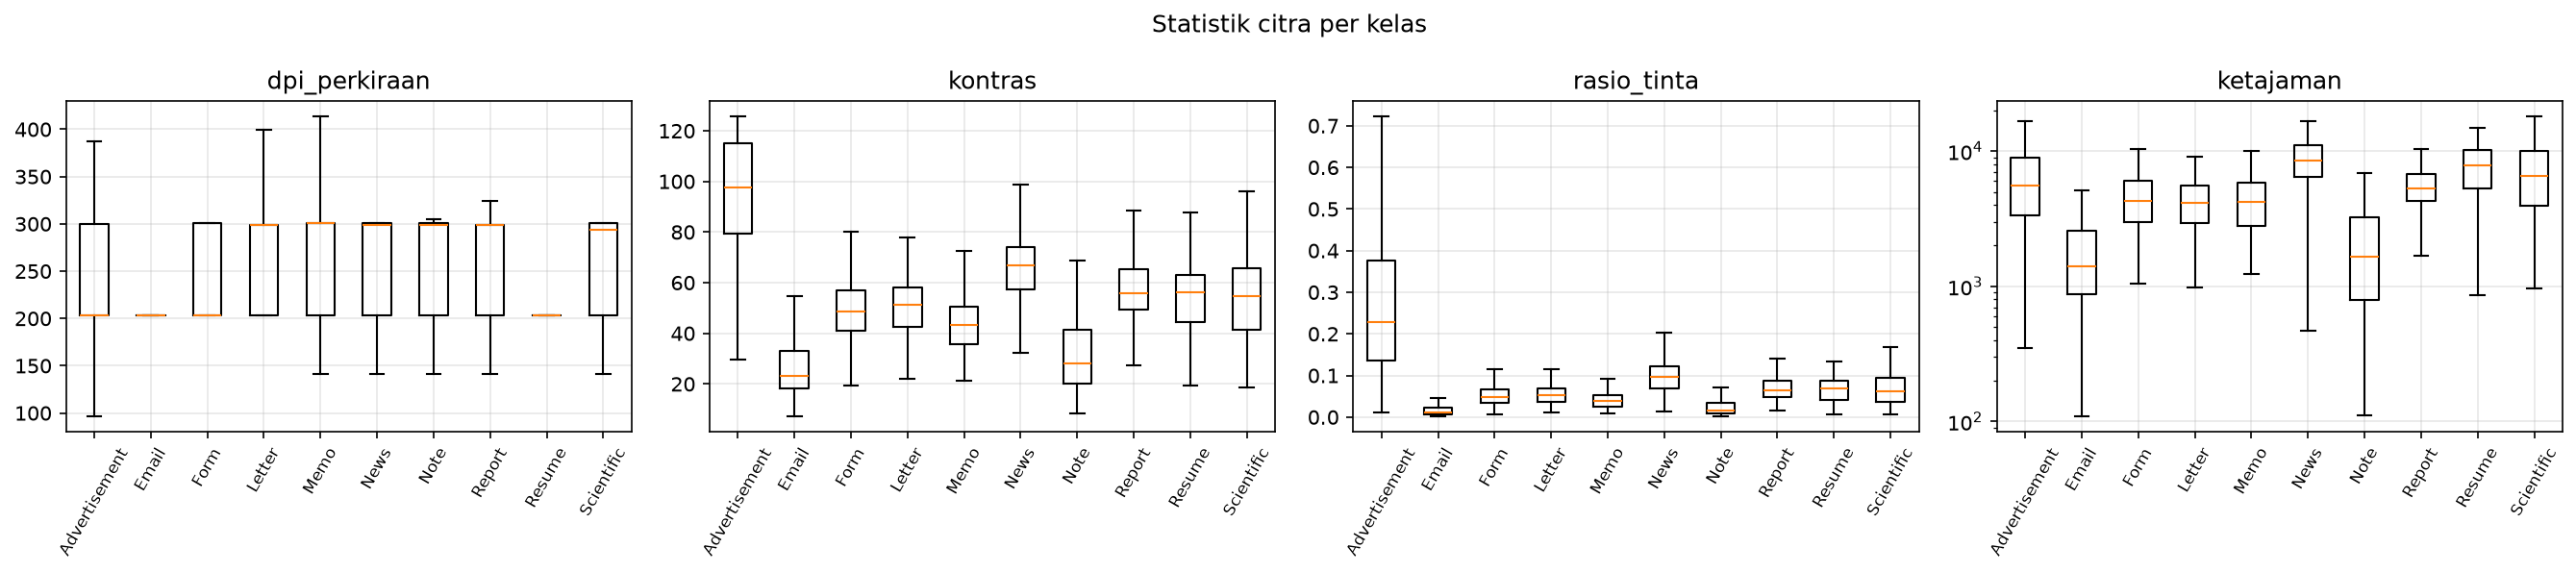
\includegraphics[width=\textwidth]{../../reports/figures/fase2_eda_statistik_citra.png}
  \caption{Statistik citra per kelas: perkiraan dpi, kontras, rasio tinta, dan ketajaman
  (variansi Laplacian, skala log)}
  \label{fig:eda-citra}
\end{figure}

Gambar~\ref{fig:eda-citra} memperlihatkan tiga hal.
\begin{enumerate}
  \item \textbf{Resolusi tidak seragam antar-kelas.} Seluruh halaman Email dan Resume
  berada di 203 dpi, sedangkan kelas lain menyebar antara 203 dan 300 dpi. Resolusi asli
  hilang setelah citra diubah ke $384\times384$, tetapi pola ini menunjukkan kelas-kelas
  itu dipindai dengan cara berbeda, sehingga menjadi sumber bias yang potensial.
  \item \textbf{Advertisement jauh lebih gelap.} Kontras dan rasio tintanya paling tinggi
  (median rasio tinta sekitar 0,23, kelas lain sekitar 0,1 atau kurang), karena halaman
  iklan didominasi gambar.
  \item \textbf{Email dan Note paling jarang tintanya}, sehingga ketajamannya juga paling
  rendah. Variansi Laplacian bergantung pada jumlah tepi, jadi halaman yang sedikit
  tulisannya otomatis mendapat skor rendah walaupun tidak kabur.
\end{enumerate}

\textit{Linear probe} (regresi logistik) di atas fitur MobileNetV2 ImageNet tanpa
\textit{fine-tune} mencapai \textbf{OA 0,7293} dan macro F1 0,7099, padahal menebak kelas
mayoritas hanya 0,1782. Tata letak halaman sudah sangat informatif bahkan tanpa pelatihan
khusus dokumen. Pada proyeksi t-SNE (Gambar~\ref{fig:eda-tsne}, kiri), Email,
Advertisement, Form, News, Resume, dan Scientific membentuk kelompok yang jelas, sedangkan
Letter, Memo, dan Report bercampur di tengah. Ketiganya adalah dokumen ketikan
berparagraf dengan tata letak yang mirip.

\subsubsection{Modalitas Teks}

Teks QS-OCR berpanjang median 174 kata per dokumen (rata-rata 224, maksimum 1.579).
Sebanyak 1,1\% dokumen tidak berisi satu pun kata, dan 7,8\% lebih panjang dari 500 kata
sehingga terpotong saat masuk CNN~1D. Laju OOV (Persamaan~\ref{eq:oov}) bermedian 5,5\%
dan rata-rata 9,8\%. Angka ini batas bawah galat OCR, dan tidak dapat dibandingkan dengan
$\pm$26\% yang dilaporkan \textcite{audebert2020}, yang memakai kamus lebih ketat.

Masalah teks terpusat di dua kelas (Tabel~\ref{tab:eda-penanda}). Ambang penanda diambil
dari ekor distribusi data (persentil 5 atau 95): teks pendek $\leq 23$ kata dan OOV tinggi
$\geq 0{,}369$.

\begin{table}[H]
  \centering
  \caption{Persentase dokumen bertanda masalah teks per kelas (QS-OCR)}
  \label{tab:eda-penanda}
  \fontsize{10}{12}\selectfont
  \begin{tabular}{|l|r|r|r|}
    \hline
    \textbf{Kelas} & \textbf{Teks kosong} & \textbf{Teks pendek} & \textbf{OOV tinggi} \\ \hline
    Note & 14,4\% & 41,3\% & 30,8\% \\ \hline
    Advertisement & 3,5\% & 17,4\% & 13,0\% \\ \hline
    Form & 0\% & 1,4\% & 10,7\% \\ \hline
    News & 0\% & 2,1\% & 8,0\% \\ \hline
    Kelas lain & 0\% & $\leq 4{,}2$\% & $\leq 3{,}4$\% \\ \hline
    \textbf{Semua} & 1,1\% & 4,7\% & 4,9\% \\ \hline
  \end{tabular}
\end{table}

Note berisi banyak tulisan tangan dan catatan pendek, sedangkan iklan sering berteks
sedikit atau dipindai terputar $90^\circ$, yang tidak dikenali Tesseract dengan
\texttt{-{}-psm 3}. Kata dengan bobot TF-IDF tertinggi per kelas
(Tabel~\ref{tab:eda-tfidf}) menunjukkan bahwa teks OCR tetap membawa penanda kelas yang
kuat. Kelas Note lagi-lagi berbeda: daftarnya berisi potongan kata rusak seperti
\texttt{ore} dan \texttt{ous}.

\begin{table}[H]
  \centering
  \caption{Kata TF-IDF tertinggi per kelas (bagian latih seed 42, QS-OCR)}
  \label{tab:eda-tfidf}
  \fontsize{10}{12}\selectfont
  \begin{tabularx}{\textwidth}{|l|>{\raggedright\arraybackslash}X|}
    \hline
    \textbf{Kelas} & \textbf{Kata khas} \\ \hline
    Advertisement & warning, surgeon, cigarette, general, advertisement, smoking, tar, nicotine \\ \hline
    Email & sent, subject, message, original, wednesday, date, thanks, meeting \\ \hline
    Form & date, fax, number, pages, form, total, morris \\ \hline
    Letter & tobacco, dear, research, new, sincerely, york \\ \hline
    Memo & correspondence, attached, philip, morris, memorandum \\ \hline
    News & said, smoking, health, smoke, tobacco, smokers \\ \hline
    Note & desk, information, james, ore, web, ous \\ \hline
    Report & tobacco, smoking, cigarette, products \\ \hline
    Resume & university, research, biology, assistant, professor \\ \hline
    Scientific & cell, cells, research, results, study, induced \\ \hline
  \end{tabularx}
\end{table}

\textit{Linear probe} di atas rata-rata vektor FastText mencapai \textbf{OA 0,6685} (macro
F1 0,6491), di bawah citra tetapi jauh di atas kelas mayoritas. Pada t-SNE
(Gambar~\ref{fig:eda-tsne}, kanan), Resume dan Email membentuk kelompok yang sangat jelas,
Scientific mengelompok di bagian atas, dan Form di sisi kanan. Pola pengelompokannya
berbeda dari citra.

\begin{figure}[H]
  \centering
  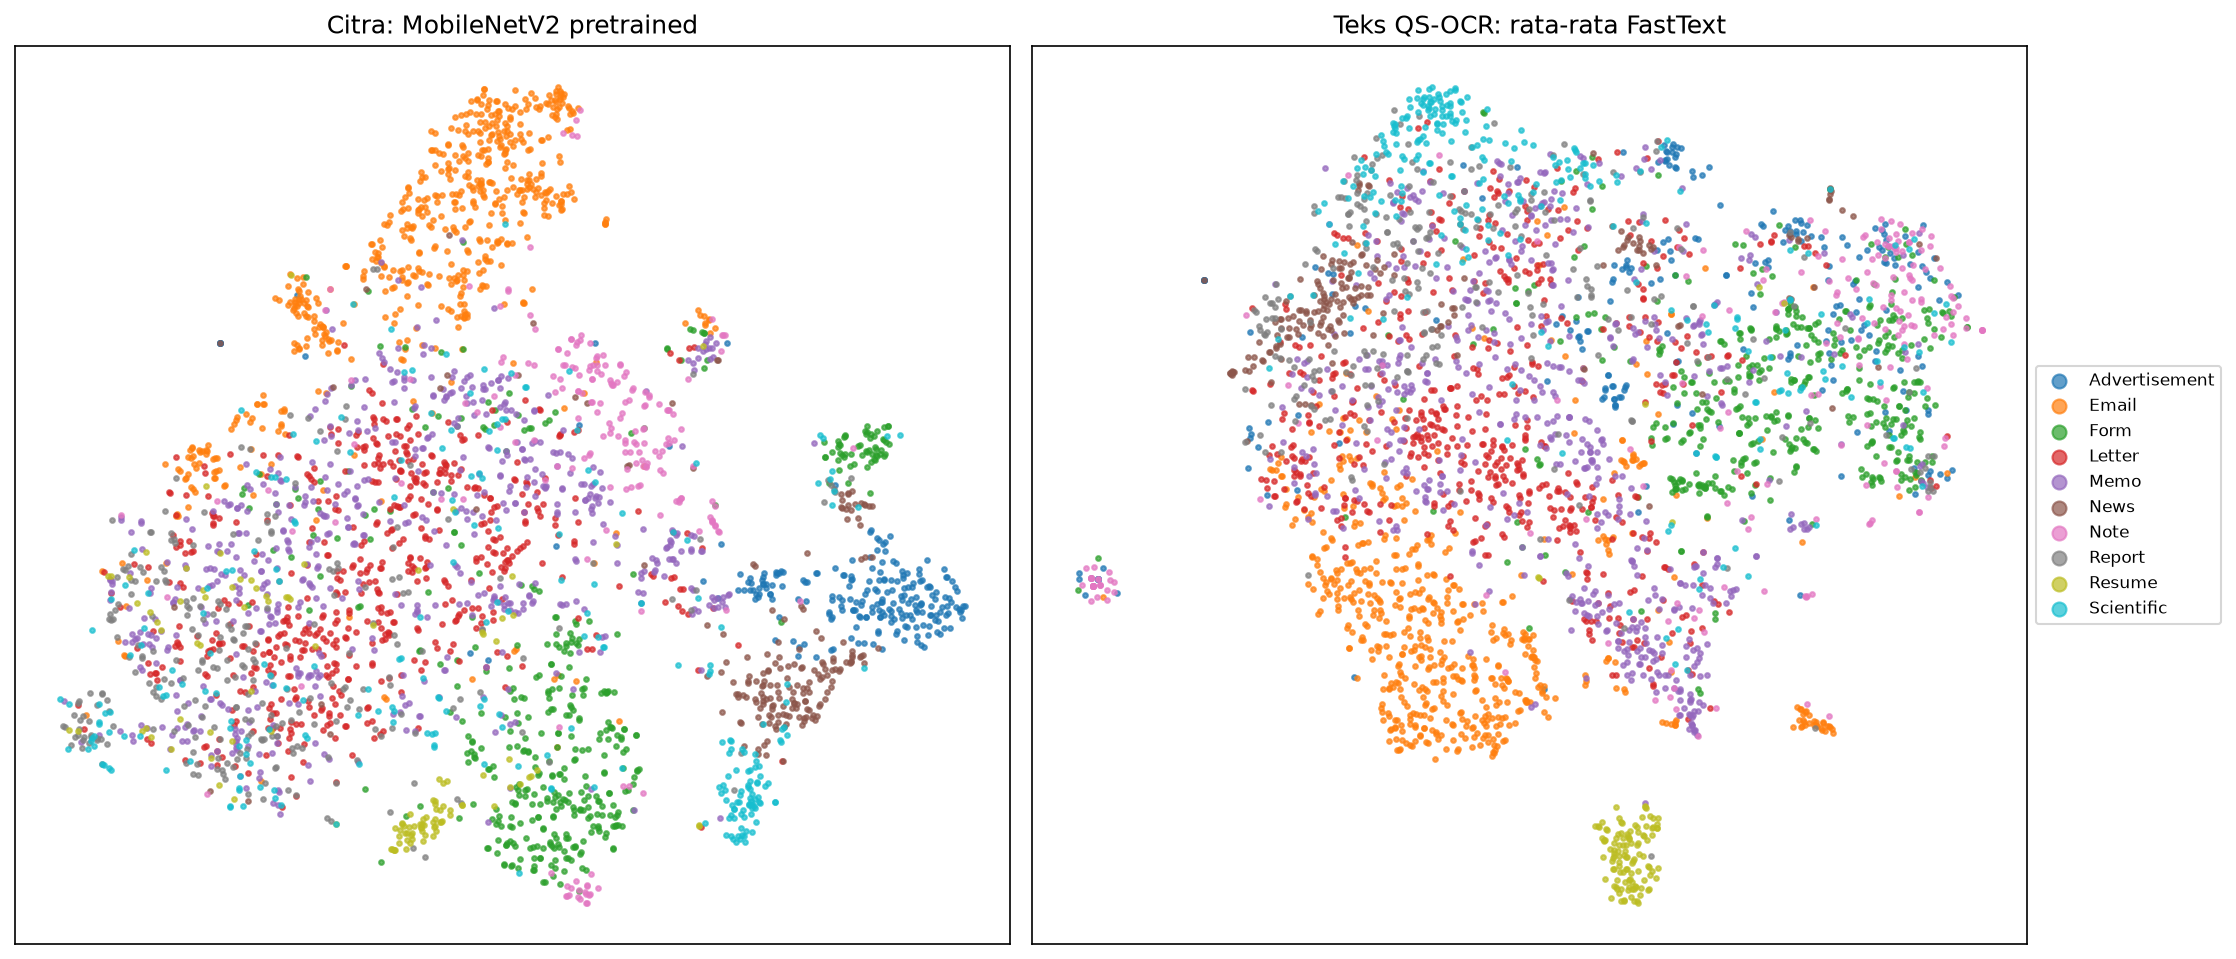
\includegraphics[width=\textwidth]{../../reports/figures/fase2_eda_tsne.png}
  \caption{Proyeksi t-SNE fitur citra (kiri, MobileNetV2 ImageNet) dan fitur teks
  (kanan, rata-rata FastText QS-OCR), diwarnai menurut kelas}
  \label{fig:eda-tsne}
\end{figure}

\subsubsection{Komplementaritas dan Kurasi}

F1 \textit{probe} per kelas memperlihatkan di mana tiap modalitas unggul
(Tabel~\ref{tab:eda-komplementer}).

\begin{table}[H]
  \centering
  \caption{F1 \textit{probe} per kelas: citra vs teks QS-OCR}
  \label{tab:eda-komplementer}
  \fontsize{10}{12}\selectfont
  \begin{tabular}{|l|c|c|c|}
    \hline
    \textbf{Kelas} & \textbf{Citra} & \textbf{Teks} & \textbf{Teks $-$ citra} \\ \hline
    Resume & 0,710 & 0,947 & $+0{,}237$ \\ \hline
    Scientific & 0,446 & 0,523 & $+0{,}077$ \\ \hline
    Email & 0,899 & 0,918 & $+0{,}019$ \\ \hline
    Memo & 0,674 & 0,627 & $-0{,}047$ \\ \hline
    Report & 0,421 & 0,366 & $-0{,}055$ \\ \hline
    News & 0,837 & 0,764 & $-0{,}073$ \\ \hline
    Form & 0,813 & 0,737 & $-0{,}076$ \\ \hline
    Letter & 0,727 & 0,624 & $-0{,}103$ \\ \hline
    Note & 0,686 & 0,397 & $-0{,}289$ \\ \hline
    Advertisement & 0,886 & 0,589 & $-0{,}297$ \\ \hline
  \end{tabular}
\end{table}

Teks unggul pada Resume, Scientific, dan Email; citra unggul jauh pada Advertisement dan
Note, tepat kelas yang teksnya paling sering kosong atau rusak. Komplementaritas ini sudah
terlihat sebelum pelatihan apa pun, dan menjadi dasar harapan bahwa fusion menolong.
Kurasi menemukan 101 dokumen Note dan 62 Advertisement yang teksnya bermasalah tetapi
citranya baik: di situlah fusion seharusnya paling berguna.

Kurasi \textbf{menandai, tidak membuang}, karena derau OCR adalah objek penelitian.
Selain penanda teks, ditemukan 12 pasangan duplikat (korelasi \textit{thumbnail} tinggi
dan dikonfirmasi kemiripan teks), dengan 1, 5, dan 4 pasangan yang terbelah antara data
latih dan uji pada seed 42, 43, dan 44. Jumlah ini terlalu kecil untuk memengaruhi
akurasi atas 2.682 dokumen uji secara berarti. Jalan pintas kode ID arsip
\parencite{larson2025} juga diuji: classifier yang hanya diberi tiga digit awal kode ID
dalam teks OCR mencapai OA 0,2782, sepuluh poin di atas kelas mayoritas tetapi jauh di
bawah \textit{probe} teks.

Probe yang sama pada keempat kondisi OCR menghasilkan PaddleOCR 0,6864, QS-OCR 0,6685,
EasyOCR 0,6521, dan Tesseract 0,6499. Urutan ini nantinya cocok dengan urutan akurasi
cabang teks yang dilatih (Subbagian~\ref{sec:hasil-teks}).

\subsection{Kualitas Keluaran OCR}\label{sec:hasil-ocr}

Proksi kualitas setiap kondisi disajikan pada Tabel~\ref{tab:proksi}.

\begin{table}[H]
  \centering
  \caption{Proksi kualitas OCR per kondisi (seluruh 3.482 halaman)}
  \label{tab:proksi}
  \fontsize{10}{12}\selectfont
  \begin{tabular}{|l|r|r|r|r|r|}
    \hline
    \textbf{Kondisi} & \textbf{\makecell{Kata/halaman\\(median)}} &
    \textbf{\makecell{Halaman\\kosong}} & \textbf{\makecell{OOV\\median}} &
    \textbf{\makecell{OOV\\rata-rata}} & \textbf{\makecell{Jaccard\\ke QS-OCR}} \\ \hline
    QS-OCR & 160 & 1,06\% & 0,055 & 0,098 & 1 \\ \hline
    Tesseract & 161 & 0,60\% & 0,057 & 0,115 & 0,920 \\ \hline
    EasyOCR & 157 & 0,17\% & 0,136 & 0,232 & 0,693 \\ \hline
    PaddleOCR & 162 & 0,06\% & 0,054 & 0,124 & 0,864 \\ \hline
  \end{tabular}
\end{table}

PaddleOCR menghasilkan teks paling lengkap: halaman kosongnya hampir nol dan OOV
mediannya terendah, walaupun dibaca dari JPG. EasyOCR menonjol ke arah sebaliknya, dengan
OOV median 2,5 kali mesin lain dan kesepakatan terendah dengan semua mesin (Jaccard 0,69
sampai 0,73). Tesseract-JPG paling dekat dengan QS-OCR, wajar karena mesinnya sekeluarga.
Untuk semua mesin, kelas dengan OOV tertinggi adalah Note (median 0,25 sampai 0,64),
disusul Advertisement dan News.

Biayanya sangat berbeda: EasyOCR di GPU 4~GB sekitar 22 kali lebih lambat daripada
Tesseract di CPU (Tabel~\ref{tab:waktu}).

\subsection{Pengaruh Mesin OCR terhadap Cabang Teks (RM1)}\label{sec:hasil-teks}

Akurasi cabang teks per kondisi disajikan pada Tabel~\ref{tab:teks}, dan uji
McNemar-nya pada Tabel~\ref{tab:mcnemar-ocr}.

\begin{table}[H]
  \centering
  \caption{Akurasi cabang teks (FastText + CNN~1D) per kondisi OCR}
  \label{tab:teks}
  \fontsize{10}{12}\selectfont
  \begin{tabular}{|l|c|c|c|}
    \hline
    \textbf{Kondisi} & \textbf{OA} & \textbf{Macro F1} & \textbf{OA per seed (42/43/44)} \\ \hline
    QS-OCR & $0{,}7266 \pm 0{,}0059$ & $0{,}7017 \pm 0{,}0053$ & 0,7345 / 0,7248 / 0,7204 \\ \hline
    Tesseract & $0{,}6970 \pm 0{,}0047$ & $0{,}6547 \pm 0{,}0083$ & 0,6913 / 0,7028 / 0,6969 \\ \hline
    EasyOCR & $0{,}7155 \pm 0{,}0061$ & $0{,}6862 \pm 0{,}0095$ & 0,7155 / 0,7081 / 0,7230 \\ \hline
    PaddleOCR & $\mathbf{0{,}7514 \pm 0{,}0043}$ & $\mathbf{0{,}7200 \pm 0{,}0057}$ &
    0,7498 / 0,7573 / 0,7472 \\ \hline
  \end{tabular}
\end{table}

\begin{table}[H]
  \centering
  \caption{McNemar antar-kondisi OCR untuk cabang teks (Holm per seed, $\alpha = 0{,}05$)}
  \label{tab:mcnemar-ocr}
  \fontsize{10}{12}\selectfont
  \begin{tabular}{|l|c|c|}
    \hline
    \textbf{Pasangan (a $-$ b)} & \textbf{Selisih OA rerata} & \textbf{Seed signifikan} \\ \hline
    Tesseract $-$ PaddleOCR & $-0{,}0544$ & 3/3 \\ \hline
    EasyOCR $-$ PaddleOCR & $-0{,}0359$ & 3/3 \\ \hline
    QS-OCR $-$ Tesseract & $+0{,}0296$ & 3/3 \\ \hline
    QS-OCR $-$ PaddleOCR & $-0{,}0249$ & 2/3 \\ \hline
    Tesseract $-$ EasyOCR & $-0{,}0185$ & 2/3 \\ \hline
    QS-OCR $-$ EasyOCR & $+0{,}0111$ & 0/3 \\ \hline
  \end{tabular}
\end{table}

\textbf{H1 didukung.} Dengan embedding, arsitektur, pembagian data, dan hiperparameter
dikunci, mesin OCR saja menggeser OA cabang teks sebesar \textbf{5,4 poin}, dari 0,6970
(Tesseract-JPG) ke 0,7514 (PaddleOCR). Tiga pasangan berbeda nyata di ketiga seed. Selisih
terbesar sekitar 11 kali simpangan baku antar-seed cabang teks. Dugaan arah juga benar:
QS-OCR mengungguli Tesseract-JPG di ketiga seed.

Tiga pengamatan menyertai hasil ini.

\textbf{Mesin lebih menentukan daripada sumber citra.} PaddleOCR yang membaca JPG
mengalahkan QS-OCR yang dibaca dari TIF asli (+2,5 poin, nyata di dua seed), sedangkan
Tesseract pada JPG kalah dari QS-OCR ($-3{,}0$ poin, nyata di tiga seed). Teks QS-OCR yang
selama ini dipakai sebagai acuan karena itu bukan batas atas.

\textbf{Proksi OOV tidak meramalkan kegunaan teks.} EasyOCR memiliki OOV terburuk dan
kesepakatan terendah, tetapi cabang teksnya lebih akurat daripada Tesseract-JPG.
Sebaliknya, \textit{linear probe} tanpa pelatihan pada rata-rata vektor FastText
meramalkan urutan mesin dengan cukup baik: PaddleOCR 0,686 $>$ QS-OCR 0,669 $>$ EasyOCR
0,652 $\approx$ Tesseract 0,650. Untuk memilih mesin OCR bagi tugas klasifikasi, probe
kecil lebih berguna daripada statistik OOV.

\textbf{Tidak ada mesin yang terbaik di semua kelas.} Keunggulan PaddleOCR tersebar di
kelas yang kaya teks: terhadap QS-OCR, F1 Advertisement naik 8,5 poin, Letter 7,4,
Report 5,1, dan Memo 4,5. Namun F1 Note \emph{turun} 9,2 poin (0,621 ke 0,529). Note
adalah kelas dengan OOV tertinggi untuk semua mesin, dan 48,3\% halamannya berisi kurang
dari 20 kata.

\subsection{Fusion per Kondisi OCR (RM3)}\label{sec:hasil-fusion}

Hasil utama disajikan pada Tabel~\ref{tab:utama} dan Gambar~\ref{fig:grid}.

\begin{table}[H]
  \centering
  \caption{OA rerata $\pm$ simpangan baku antar-seed per kondisi OCR}
  \label{tab:utama}
  \fontsize{9}{11}\selectfont
  \setlength{\tabcolsep}{3.5pt}
  \begin{tabular}{|l|c|c|c|c|c|}
    \hline
    \textbf{Kondisi} & \textbf{IMAGE} & \textbf{TEXT} & \textbf{LATE} & \textbf{CONCAT} &
    \textbf{ORACLE} \\ \hline
    QS-OCR & $0{,}8169 \pm 0{,}0257$ & $0{,}7266 \pm 0{,}0059$ & $0{,}8456 \pm 0{,}0221$ &
    $0{,}8316 \pm 0{,}0119$ & $0{,}9023 \pm 0{,}0127$ \\ \hline
    Tesseract & $0{,}8169 \pm 0{,}0257$ & $0{,}6970 \pm 0{,}0047$ & $0{,}8376 \pm 0{,}0174$ &
    $0{,}8349 \pm 0{,}0102$ & $0{,}8950 \pm 0{,}0086$ \\ \hline
    EasyOCR & $0{,}8169 \pm 0{,}0257$ & $0{,}7155 \pm 0{,}0061$ & $0{,}8538 \pm 0{,}0158$ &
    $0{,}8567 \pm 0{,}0034$ & $0{,}8972 \pm 0{,}0091$ \\ \hline
    PaddleOCR & $0{,}8169 \pm 0{,}0257$ & $0{,}7514 \pm 0{,}0043$ &
    $\mathbf{0{,}8653 \pm 0{,}0122}$ & $\mathbf{0{,}8674 \pm 0{,}0014}$ &
    $0{,}9079 \pm 0{,}0105$ \\ \hline
  \end{tabular}
\end{table}

\begin{figure}[H]
  \centering
  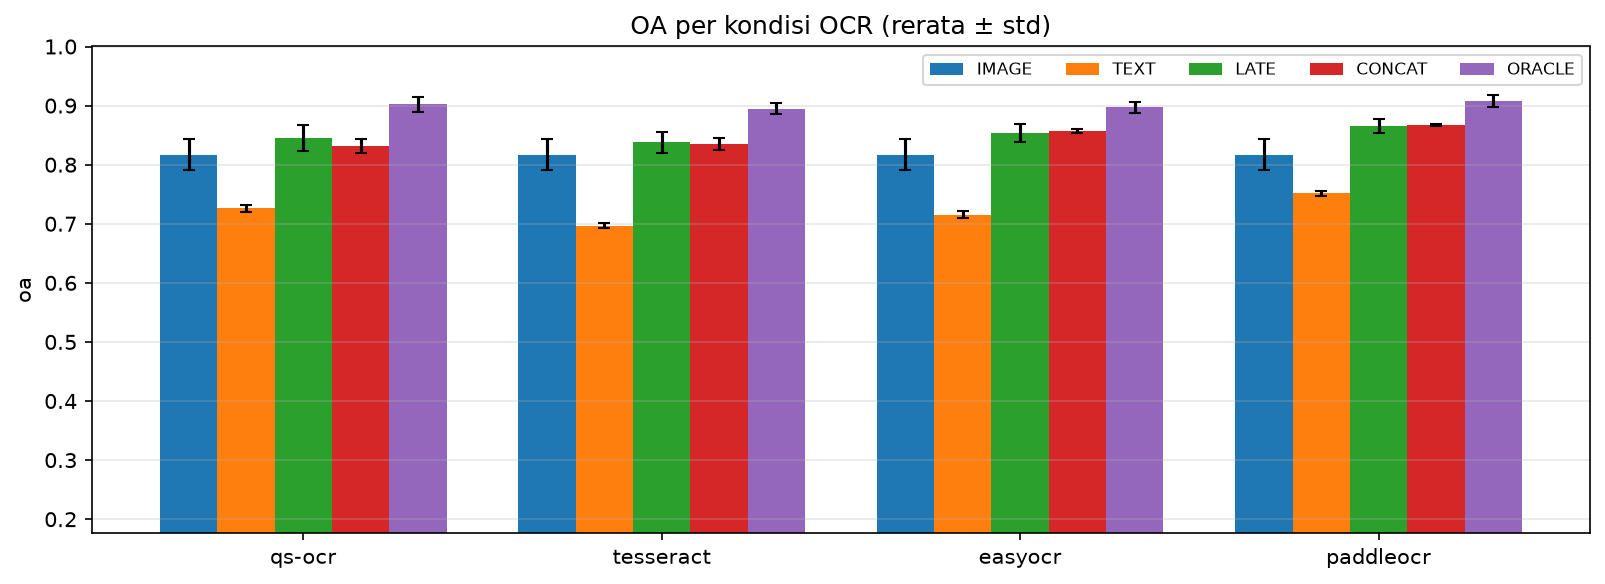
\includegraphics[width=\textwidth]{../../reports/figures/fase2_grid_oa.png}
  \caption{OA per kondisi OCR, rerata $\pm$ simpangan baku tiga seed}
  \label{fig:grid}
\end{figure}

\textbf{OCR yang lebih baik menaikkan fusion, untuk kedua aturan.} Dari Tesseract-JPG ke
PaddleOCR, LATE naik 2,8 poin dan CONCAT 3,2 poin, berbeda nyata di ketiga seed. Sel
terbaik adalah \textbf{CONCAT dengan PaddleOCR, $0{,}8674 \pm 0{,}0014$} (macro F1
$0{,}8524 \pm 0{,}0016$), 3,3 poin di atas fusion \textit{end-to-end} Fase~1 (0,8342).
Macro F1 mengikuti pola yang sama dengan OA.

Seberapa banyak potensi teks dipanen fusion (Persamaan~\ref{eq:panen}) disajikan pada
Tabel~\ref{tab:panen}. Sebagai pembanding, fusion \textcite{audebert2020} memanen 43\%
potensinya, dan fusion \textit{end-to-end} Fase~1 29\%.

\begin{table}[H]
  \centering
  \caption{Potensi oracle dan bagian yang dipanen fusion (rerata seed)}
  \label{tab:panen}
  \fontsize{10}{12}\selectfont
  \begin{tabular}{|l|c|c|c|c|c|}
    \hline
    \textbf{Kondisi} & \textbf{Potensi} & \textbf{LATE $-$ IMAGE} & \textbf{Panen LATE} &
    \textbf{CONCAT $-$ IMAGE} & \textbf{Panen CONCAT} \\ \hline
    QS-OCR & 0,0854 & $+0{,}0287$ & 34\% & $+0{,}0147$ & 13\% \\ \hline
    Tesseract & 0,0781 & $+0{,}0206$ & 25\% & $+0{,}0180$ & 19\% \\ \hline
    EasyOCR & 0,0803 & $+0{,}0369$ & 46\% & $+0{,}0398$ & 46\% \\ \hline
    PaddleOCR & 0,0910 & $+0{,}0483$ & 52\% & $+0{,}0505$ & 52\% \\ \hline
  \end{tabular}
\end{table}

LATE berada di atas IMAGE di 12 dari 12 sel (minimum $+0{,}006$). CONCAT tidak: pada
QS-OCR seed 43, CONCAT 0,8188 berada di bawah IMAGE 0,8386.

\textbf{H3a didukung untuk LATE, lemah untuk CONCAT.} Korelasi Spearman antara OA cabang
teks dan $\Delta_\text{teks}$ LATE adalah 0,683 atas 12 sel; terhadap kenaikan LATE di
atas IMAGE 0,517, dan terhadap panen LATE 0,65. Untuk CONCAT, $\Delta_\text{teks}$ dengan
pengganti kosong tidak sah sebagai ukuran (Subbagian~\ref{sec:hasil-missing}), sehingga
yang dipakai adalah kenaikan di atas IMAGE; korelasinya hanya 0,287. Akurasi teks juga
bukan satu-satunya penentu: cabang teks EasyOCR lebih lemah daripada QS-OCR, tetapi
dipanen jauh lebih banyak (46\% vs 34\% untuk LATE, 46\% vs 13\% untuk CONCAT).

\textbf{H3b tidak didukung; arahnya justru terbalik bila cabang citra lemah.} Hasil
McNemar LATE vs CONCAT disajikan pada Tabel~\ref{tab:late-concat}.

\begin{table}[H]
  \centering
  \caption{McNemar LATE vs CONCAT per kondisi (Holm per seed); \enquote{--} berarti tidak
  berbeda nyata}
  \label{tab:late-concat}
  \fontsize{10}{12}\selectfont
  \begin{tabular}{|c|c|c|c|c|c|}
    \hline
    \textbf{Seed} & \textbf{IMAGE} & \textbf{QS-OCR} & \textbf{Tesseract} & \textbf{EasyOCR} &
    \textbf{PaddleOCR} \\ \hline
    42 & 0,8315 & LATE lebih baik & -- & -- & -- \\ \hline
    43 & 0,8386 & LATE lebih baik & -- & -- & LATE lebih baik \\ \hline
    44 & 0,7808 & CONCAT lebih baik & -- & CONCAT lebih baik & CONCAT lebih baik \\ \hline
  \end{tabular}
\end{table}

Rerata kedua aturan hampir sama (selisih paling besar 1,4 poin), dan pemenangnya
bergantung pada kekuatan cabang citra. LATE unggul nyata saat cabang citra kuat (seed 42
dan 43), sedangkan CONCAT unggul nyata di tiga dari empat kondisi saat cabang citra lemah
(seed 44). Rata-rata tanpa bobot ikut jatuh bersama cabang yang lemah, sedangkan
\textit{head} yang dilatih menyesuaikan bobotnya. CONCAT juga jauh lebih stabil
antar-seed (simpangan baku 0,0014 sampai 0,0119, LATE 0,0122 sampai 0,0221). Untuk cabang
\emph{teks} yang lemah (Tesseract-JPG), kedua aturan tidak berbeda nyata di seed mana pun.

Matriks konfusi sel terbaik ditunjukkan Gambar~\ref{fig:konfusi}. Kelas tersulit tetap
Scientific (\textit{recall} 0,46), yang terutama tertukar dengan Report dan Form, sama
dengan pola pada ketiga paper rujukan.

\begin{figure}[H]
  \centering
  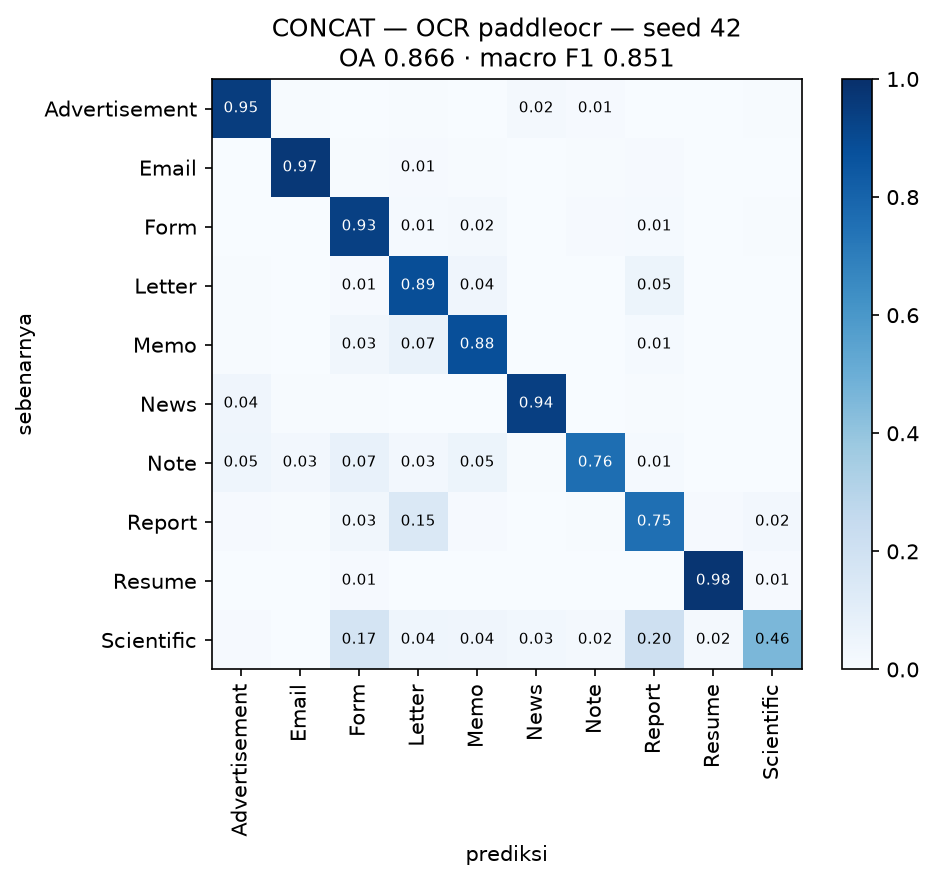
\includegraphics[width=0.72\textwidth]{../../reports/figures/fase2_konfusi_terbaik.png}
  \caption{Matriks konfusi ternormalisasi per baris, CONCAT dengan PaddleOCR, seed 42}
  \label{fig:konfusi}
\end{figure}

\subsection{Uji \textit{Missing Modality}}\label{sec:hasil-missing}

\subsubsection{Pengganti kosong: anomali}

Hasil uji dengan pengganti kosong, yang dirancang sebelum eksekusi, disajikan pada
Tabel~\ref{tab:missing-kosong}.

\begin{table}[H]
  \centering
  \caption{Uji \textit{missing modality} dengan pengganti kosong: selisih OA terhadap model
  unimodal modalitas yang tersisa (rerata seed)}
  \label{tab:missing-kosong}
  \fontsize{10}{12}\selectfont
  \begin{tabular}{|l|c|c|c|c|}
    \hline
    \textbf{Kondisi} & \textbf{\makecell{LATE tanpa teks\\$-$ IMAGE}} &
    \textbf{\makecell{CONCAT tanpa teks\\$-$ IMAGE}} &
    \textbf{\makecell{LATE tanpa citra\\$-$ TEXT}} &
    \textbf{\makecell{CONCAT tanpa citra\\$-$ TEXT}} \\ \hline
    QS-OCR & $-0{,}022$ & $-0{,}563$ & $-0{,}268$ & $-0{,}112$ \\ \hline
    Tesseract & $-0{,}008$ & $-0{,}591$ & $-0{,}271$ & $-0{,}135$ \\ \hline
    EasyOCR & $-0{,}001$ & $-0{,}137$ & $-0{,}337$ & $-0{,}202$ \\ \hline
    PaddleOCR & $-0{,}003$ & $-0{,}301$ & $-0{,}349$ & $-0{,}216$ \\ \hline
  \end{tabular}
\end{table}

Hanya LATE tanpa teks yang berperilaku seperti seharusnya: ia mendarat di IMAGE (selisih
paling besar 2,2 poin). CONCAT tanpa teks jatuh \textbf{jauh di bawah cabang citra
sendiri}, sampai 59 poin, dan semua versi tanpa citra jatuh di bawah cabang teks sendiri.
Kehilangan satu modalitas tidak mungkin lebih buruk daripada model unimodal modalitas yang
tersisa, kecuali penggantinya keluar distribusi bagi model. Dugaan awal kami untuk CONCAT
adalah bahwa \textit{head} belajar \enquote{teks kosong $\Rightarrow$ Note}, karena
sebagian halaman Note pada QS-OCR kosong. Dua dugaan ini diuji pada uji lanjutan (H4a dan
H4b).

\subsubsection{Uji lanjutan: pengganti rerata dan \textit{head} tanpa teks kosong}

Dokumen yang kosong menurut model berjumlah 27 (QS-OCR: 20 Note, 7 Advertisement), 11
(Tesseract: 6 Note, 5 Advertisement), dan 0 untuk EasyOCR maupun PaddleOCR. Di bagian latih
\textit{head} terdapat 4 sampai 8 dokumen kosong untuk QS-OCR dan 2 sampai 4 untuk
Tesseract, dari 720 dokumen. Hasil uji lanjutan disajikan pada Tabel~\ref{tab:missing-lanjutan}.

\begin{table}[H]
  \centering
  \caption{Uji lanjutan: selisih OA terhadap model unimodal modalitas yang tersisa (rerata
  seed)}
  \label{tab:missing-lanjutan}
  \fontsize{10}{12}\selectfont
  \begin{tabularx}{\textwidth}{|>{\raggedright\arraybackslash}X|c|c|c|c|}
    \hline
    \textbf{Selisih} & \textbf{QS-OCR} & \textbf{Tesseract} & \textbf{EasyOCR} &
    \textbf{PaddleOCR} \\ \hline
    CONCAT tanpa teks, kosong $-$ IMAGE & $-0{,}563$ & $-0{,}591$ & $-0{,}137$ & $-0{,}301$ \\ \hline
    CONCAT tanpa teks, rerata $-$ IMAGE & $-0{,}108$ & $-0{,}130$ & $-0{,}026$ & $-0{,}027$ \\ \hline
    CONCAT\_nonkosong tanpa teks, kosong $-$ IMAGE & $-0{,}496$ & $-0{,}633$ & $-0{,}137$ & $-0{,}301$ \\ \hline
    LATE tanpa teks, rerata $-$ IMAGE & $-0{,}132$ & $-0{,}129$ & $-0{,}076$ & $-0{,}074$ \\ \hline
    LATE tanpa citra, rerata $-$ TEXT & $-0{,}029$ & $-0{,}036$ & $-0{,}040$ & $-0{,}042$ \\ \hline
    CONCAT tanpa citra, rerata $-$ TEXT & $-0{,}005$ & $+0{,}006$ & $-0{,}017$ & $-0{,}014$ \\ \hline
    CONCAT\_nonkosong $-$ CONCAT (masukan lengkap) & $+0{,}006$ & $+0{,}003$ & 0 & 0 \\ \hline
  \end{tabularx}
\end{table}

\textbf{H4a didukung sebagian.} Dengan pengganti rerata, kedua aturan tanpa citra
mendarat paling jauh 4,2 poin di bawah cabang teks, padahal dengan pengganti kosong 11
sampai 35 poin. Kejatuhan tanpa citra karena itu artefak pengganti. CONCAT tanpa teks pulih
sebagian besar (QS-OCR $-0{,}563 \rightarrow -0{,}108$; Tesseract
$-0{,}591 \rightarrow -0{,}130$) dan mendarat dekat IMAGE pada EasyOCR dan PaddleOCR
($-0{,}026$ dan $-0{,}027$). Pada QS-OCR dan Tesseract masih tersisa 11 sampai 13 poin di
bawah IMAGE, dengan sebaran besar antar-seed ($-0{,}03$ sampai $-0{,}20$). Pada kedua
kondisi itu, \textit{head} memang tidak dapat bekerja setara cabang citra tanpa teks.

\textbf{H4b tidak didukung.} Prasyaratnya terpenuhi: membuang dokumen kosong hanya
menggeser CONCAT dengan masukan lengkap 0,3 sampai 0,6 poin. Kriteria (i) juga terpenuhi:
dengan teks kosong, porsi prediksi Note membengkak dari 0,058 (porsi sebenarnya) menjadi
0,727, 0,756, 0,192, dan 0,320 (QS-OCR, Tesseract, EasyOCR, PaddleOCR). Namun kriteria (ii)
gagal di keempat kondisi. \textit{Head} tanpa dokumen kosong tetap menarik prediksi ke Note
(0,483 pada QS-OCR, bahkan naik ke 0,817 pada Tesseract). Bukti paling langsung datang
dari EasyOCR dan PaddleOCR: tidak ada satu pun dokumen kosong pada kedua kondisi itu, tetapi
tarikan ke Note tetap muncul. Dengan pengganti rerata, porsi Note kembali normal (0,04
sampai 0,09 per sel). Tarikan itu karena itu milik vektor teks kosong, bukan hasil belajar
dari dokumen kosong di data latih. Dugaan yang tersisa, dan belum diuji, adalah bahwa Note
sebagai kelas berteks terpendek memiliki fitur yang paling dekat dengan fitur teks kosong,
sehingga \textit{head} berekstrapolasi ke arah Note. Besar tarikannya berubah tajam
antar-seed (PaddleOCR: 0,044 / 0,532 / 0,383), sesuai dengan ekstrapolasi di luar
distribusi.

\textbf{Pengganti rerata tidak netral untuk LATE.} LATE tanpa teks dengan pengganti kosong
mendarat di IMAGE, tetapi dengan rerata logit latih ia jatuh 7 sampai 13 poin di bawah
IMAGE (negatif di setiap sel). Rerata logit menambahkan bias kelas tetap ke logit citra,
dan logit latih cabang teks berasal dari model yang dilatih pada dokumen itu sendiri.
Jadi, pengganti yang sah berbeda menurut aturan: pengganti kosong untuk LATE tanpa teks,
pengganti rerata untuk CONCAT tanpa teks dan untuk semua versi tanpa citra.

\subsection{Posisi terhadap Literatur}\label{sec:posisi-hasil}

Tabel~\ref{tab:literatur} menempatkan hasil ini di samping studi rujukan.

\begin{table}[H]
  \centering
  \caption{OA fusion pada Tobacco3482 dan protokolnya}
  \label{tab:literatur}
  \fontsize{10}{12}\selectfont
  \begin{tabularx}{\textwidth}{|>{\raggedright\arraybackslash}X|>{\raggedright\arraybackslash}p{6.2cm}|c|}
    \hline
    \textbf{Studi} & \textbf{Protokol} & \textbf{OA fusion} \\ \hline
    \textcite{kashyap2026} & dilatih pada RVL-CDIP, Tobacco3482 hanya diuji & 0,9200 \\ \hline
    \textcite{audebert2020} & 800 dokumen latih, tiga run & 0,878 \\ \hline
    Fase~1 (replikasi Audebert) & 800 dokumen latih, tiga seed & $0{,}8342 \pm 0{,}0105$ \\ \hline
    \textbf{Penelitian ini, CONCAT + PaddleOCR} & 800 dokumen latih, tiga seed &
    $\mathbf{0{,}8674 \pm 0{,}0014}$ \\ \hline
  \end{tabularx}
\end{table}

Angka antarbaris tidak sepenuhnya sebanding. \textcite{kashyap2026} melatih pada
$\pm$320.000 dokumen RVL-CDIP, dan angka Tobacco3482-nya tidak konsisten dengan
protokolnya sendiri (Subbagian~\ref{sec:kajian-pustaka}). Yang sebanding langsung adalah
dua baris terakhir: dengan data dan pembagian yang sama, mengganti mesin OCR dan aturan
fusion menaikkan fusion 3,3 poin dan memperkecil simpangan baku antar-seed tujuh kali lipat.


% ------------------------------------------------------------- akhir
\daftarreferensi

\appendix
\chapter{Riwayat Pemilihan Referensi dan Tanggapan Dosen}\label{lam:riwayat}

\section*{A.1 Pemilihan Jurnal Awal}

Jurnal pertama yang dipilih pada Progress~1 adalah \textcite{audebert2020}. Ada empat
alasan:
\begin{enumerate}
  \item \textbf{Sesuai topik mata kuliah.} Paper ini menggabungkan dua modalitas yang
  asalnya sama tetapi sifatnya berbeda: tata letak halaman dan isi tulisan.
  \item \textbf{Datanya terbuka.} Citra Tobacco3482 tersedia di Kaggle, dan teks OCR-nya
  dirilis penulis sebagai QS-OCR, sehingga modalitas teks tidak perlu dibuat sendiri.
  \item \textbf{Arsitekturnya ringan.} MobileNetV2 dan FastText dengan CNN~1D dapat
  dilatih pada GPU laptop 4~GB.
  \item \textbf{Tidak ada kode resmi.} Repositori QS-OCR hanya berisi skrip OCR, sehingga
  seluruh arsitektur harus ditulis ulang dari spesifikasi paper. Ini menuntut pemahaman
  metode, bukan sekadar menjalankan kode orang lain.
\end{enumerate}

\section*{A.2 Tanggapan Dosen atas Progress 1}

\begin{table}[H]
  \centering
  \caption{Tanggapan dosen pengampu dan tindak lanjutnya}
  \label{tab:tanggapan}
  \fontsize{10}{12}\selectfont
  \begin{tabularx}{\textwidth}{|>{\raggedright\arraybackslash}p{5.4cm}|>{\raggedright\arraybackslash}X|}
    \hline
    \textbf{Tanggapan} & \textbf{Tindak lanjut} \\ \hline
    Alur OCR $\rightarrow$ teks dengan Tesseract dan FastText sudah dipahami &
    Dipertahankan sebagai kondisi acuan (QS-OCR $\times$ FastText) \\ \hline
    Eksplorasi metode OCR: EasyOCR, PaddleOCR, Keras-OCR &
    Mesin OCR dijadikan variabel penelitian (RM1). Keras-OCR bersyarat, lihat risiko
    R3 \\ \hline
    Celah penelitian belum ditentukan &
    Dirumuskan pada Bab~\ref{bab:pendahuluan} dan Subbab~\ref{sec:kajian-pustaka}, didukung
    hasil studi pendahuluan \\ \hline
    Kemungkinan eksplorasi pada embedding &
    Embedding dijadikan variabel kedua: FastText dan BERT (RM2) \\ \hline
    Teks yang dideteksi sebagai objek, untuk tahap selanjutnya &
    Kotak posisi teks disimpan sejak langkah OCR; rancangannya pada
    Subbab~\ref{sec:lanjutan} \\ \hline
    Referensi masih tahun 2019 dan berbentuk arsip; minimal tahun 2025 &
    Referensi utama diganti ke \textcite{kashyap2026}. Audebert dikutip dari versi
    terbitnya (Springer, 2020) sebagai baseline yang telah direplikasi \\ \hline
  \end{tabularx}
  \sumber{Catatan tanggapan dosen pengampu.}
\end{table}

Satu hal perlu dicatat soal referensi. Paper Audebert sebenarnya telah terbit di ECML
PKDD 2019 Workshops, Springer CCIS vol.~1167 (2020). Kesalahan ada pada Progress~1, yang
mengutip versi arXiv. Namun tahun terbitnya tetap tidak memenuhi syarat, sehingga posisi
referensi utama tetap diganti.

\section*{A.3 Pencarian Referensi Baru}

Pencarian dilakukan melalui Crossref dan Semantic Scholar dengan empat kriteria:
\begin{enumerate}
  \item terbit di jurnal atau prosiding pada 2025 atau sesudahnya, bukan
  \textit{preprint};
  \item membahas klasifikasi dokumen multimodal teks--citra, perbandingan mesin OCR, atau
  ketahanan embedding terhadap derau OCR;
  \item metadata (DOI, volume, halaman) dapat diverifikasi;
  \item teks lengkapnya dapat dibaca, tidak hanya abstraknya.
\end{enumerate}

Hasilnya dirangkum pada Tabel~\ref{tab:referensi-baru}. Untuk \textcite{larson2025}, yang
dibaca baru abstraknya, karena unduhan teks lengkapnya belum berhasil.

\begin{table}[H]
  \centering
  \caption{Referensi utama dan pendukung yang terbit tahun 2025--2026}
  \label{tab:referensi-baru}
  \fontsize{10}{12}\selectfont
  \begin{tabularx}{\textwidth}{|l|>{\raggedright\arraybackslash}X|}
    \hline
    \textbf{Referensi} & \textbf{Peran dalam penelitian ini} \\ \hline
    \textcite{kashyap2026} & Referensi utama: fusion teks--citra terkini pada
    Tobacco3482 \\ \hline
    \textcite{mironczuk2026} & Pembingkai celah: meta-analisis 139 studi fusion untuk
    klasifikasi dokumen \\ \hline
    \textcite{francis2025} & Perbandingan Tesseract, EasyOCR, PaddleOCR, Keras-OCR, dan
    mesin lain \\ \hline
    \textcite{zhang2025} & Bukti bahwa galat OCR merambat ke tugas lanjutan \\ \hline
    \textcite{michail2025} & Ketahanan embedding terhadap derau OCR \\ \hline
    \textcite{larson2025} & Jalan pintas kode ID pada Tobacco3482 \\ \hline
  \end{tabularx}
  \sumber{Penelusuran kelompok.}
\end{table}

\section*{A.4 Mengapa Kashyap et al. sebagai Referensi Utama}

\textcite{kashyap2026} adalah penerus langsung Audebert: keduanya menggabungkan cabang
citra dan cabang teks OCR, dan keduanya diuji pada Tobacco3482. Kashyap juga
membandingkan hasilnya secara eksplisit dengan Audebert.

Paper ini \textbf{tidak direplikasi}. \textit{Fine-tuning}-nya memakan sekitar 63 jam
pada GPU 16~GB dengan RVL-CDIP, jauh di luar perangkat yang tersedia. Yang diambil dari
paper ini adalah:
\begin{itemize}
  \item embedding BERT;
  \item aturan fusion rata-rata logit;
  \item arah lanjutan yang disebut penulisnya sendiri, yaitu pembobotan modalitas adaptif
  dan kondisi degradasi OCR.
\end{itemize}
Celah yang paling menentukan adalah mesin OCR-nya yang tidak disebutkan. Catatan kritis
lengkapnya ada pada Lampiran~\ref{lam:kashyap}.

\chapter{Catatan Kritis atas Kashyap et al. (2026)}\label{lam:kashyap}

Catatan berikut disusun dari pembacaan teks lengkap \textcite{kashyap2026}.

\begin{enumerate}
  \item \textbf{Angka 92,00\% pada Tobacco3482 tidak konsisten dengan protokolnya
  sendiri.}
  \begin{itemize}
    \item Model dilatih pada 16 kelas RVL-CDIP. Penulis sendiri menyatakan bahwa kelas
    Note dan Report hanya ada di Tobacco3482.
    \item Kedua kelas itu berisi $201 + 265 = 466$ dokumen, yang tidak mungkin diprediksi
    benar oleh model 16 kelas RVL-CDIP.
    \item Bila seluruh 3.482 dokumen dievaluasi, akurasi maksimum yang mungkin adalah:
    \begin{equation}\label{eq:kashyap-maks}
      \mathrm{OA}_\text{maks} = \frac{3482 - 466}{3482} = \frac{3016}{3482} = 0{,}866
    \end{equation}
    \item Tabel per kelas paper memang hanya memuat 8 kelas.
  \end{itemize}
  Kemungkinan besar 92\% dihitung pada sekitar 3.016 dokumen, padahal tabel dataset
  paper menyebut 3.482 dokumen dan 10 kelas.
  \item \textbf{Perbandingan dengan Audebert tidak setara.} Paper menyandingkan 92,00\%
  (dilatih pada $\pm$320.000 dokumen RVL-CDIP) dengan 87,8\% Audebert (dilatih pada
  800 dokumen Tobacco3482), tanpa menyebut perbedaan protokol itu.
  \item \textbf{Potensi tumpang tindih data tidak dibahas.} RVL-CDIP dan Tobacco3482
  sama-sama diambil dari arsip industri tembakau yang sama. Hal ini belum kami verifikasi,
  karena verifikasinya membutuhkan RVL-CDIP.
  \item \textbf{Satu kali run}, tanpa simpangan baku dan tanpa uji statistik. Metrik
  Tobacco3482 dilaporkan dalam bentuk \textit{weighted}, bukan macro.
  \item \textbf{Mesin OCR tidak disebutkan}, sehingga cabang teksnya tidak dapat
  direproduksi, dan keunggulan BERT tidak dapat dipisahkan dari efek mesin OCR.
\end{enumerate}

Catatan ini tidak mengurangi nilai paper tersebut sebagai acuan arsitektur. Catatan ini
menjelaskan mengapa angka penelitian ini tidak dibandingkan langsung dengan angka
Kashyap, dan mengapa mesin OCR dijadikan variabel.

\chapter{Hasil Lengkap Studi Pendahuluan}\label{lam:hasil}

Tabel~\ref{tab:per-kelas} menyajikan F1 per kelas hasil replikasi kelompok (K), yaitu
rata-rata tiga seed, berdampingan dengan Tabel~3 \textcite{audebert2020} (P).

Selisih terbesar ada pada kelas Resume untuk model fusion: 0,803 berbanding 0,96. Selisih
inilah yang menjadi petunjuk pertama bahwa cabang teks tidak terpakai, karena model teks
saja mencapai 0,969 pada kelas yang sama.

\begin{table}[H]
  \centering
  \caption{F1 per kelas: replikasi kelompok (K) dan paper (P)}
  \label{tab:per-kelas}
  \fontsize{10}{12}\selectfont
  \begin{tabular}{|l|c|c|c|c|c|c|c|c|}
    \hline
    & \multicolumn{2}{c|}{\textbf{Teks}} & \multicolumn{2}{c|}{\textbf{Citra}} &
      \multicolumn{2}{c|}{\textbf{Fusion}} & \multicolumn{2}{c|}{\textbf{Oracle}} \\ \hline
    \textbf{Kelas} & K & P & K & P & K & P & K & P \\ \hline
    Advertisement & 0,537 & 0,60 & 0,902 & 0,94 & 0,894 & 0,93 & 0,930 & 0,94 \\ \hline
    Email         & 0,953 & 0,96 & 0,955 & 0,96 & 0,961 & 0,98 & 0,983 & 0,99 \\ \hline
    Form          & 0,718 & 0,76 & 0,804 & 0,85 & 0,848 & 0,88 & 0,902 & 0,94 \\ \hline
    Letter        & 0,671 & 0,71 & 0,805 & 0,83 & 0,835 & 0,86 & 0,898 & 0,92 \\ \hline
    Memo          & 0,758 & 0,79 & 0,844 & 0,90 & 0,879 & 0,90 & 0,920 & 0,93 \\ \hline
    News          & 0,709 & 0,67 & 0,890 & 0,89 & 0,883 & 0,90 & 0,938 & 0,93 \\ \hline
    Note          & 0,621 & 0,62 & 0,771 & 0,83 & 0,780 & 0,85 & 0,876 & 0,89 \\ \hline
    Report        & 0,495 & 0,43 & 0,527 & 0,61 & 0,638 & 0,71 & 0,735 & 0,81 \\ \hline
    Resume        & 0,969 & 0,97 & 0,784 & 0,80 & 0,803 & 0,96 & 0,951 & 0,97 \\ \hline
    Scientific    & 0,587 & 0,57 & 0,554 & 0,62 & 0,583 & 0,68 & 0,718 & 0,79 \\ \hline
    \textbf{Macro F1} & 0,702 & 0,71 & 0,784 & 0,82 & 0,811 & 0,86 & 0,885 & 0,91 \\ \hline
    \textbf{OA}       & 0,727 & 0,738 & 0,809 & 0,845 & 0,834 & 0,878 & 0,898 & 0,921 \\ \hline
  \end{tabular}
  \sumber{Eksekusi kelompok; kolom P dari \textcite{audebert2020}.}
\end{table}

Selain model di atas, studi pendahuluan juga menjalankan tiga uji lanjutan, semuanya
pada seed 42:
\begin{enumerate}
  \item fusion konkatenasi tanpa \textit{early stopping}: OA 0,8304, macro F1 0,8108;
  \item diagnostik fitur cabang teks, tanpa pelatihan;
  \item fusion yang diperbaiki: OA 0,8110, macro F1 0,8108.
\end{enumerate}
Ketiganya diringkas pada Subbab~\ref{sec:studi-pendahuluan}.

\end{document}
